\section*{Answer 2}
\label{answer-2}

\vspace*{\fill}
\begin{figure}[h] % SS of TM
  \centering
  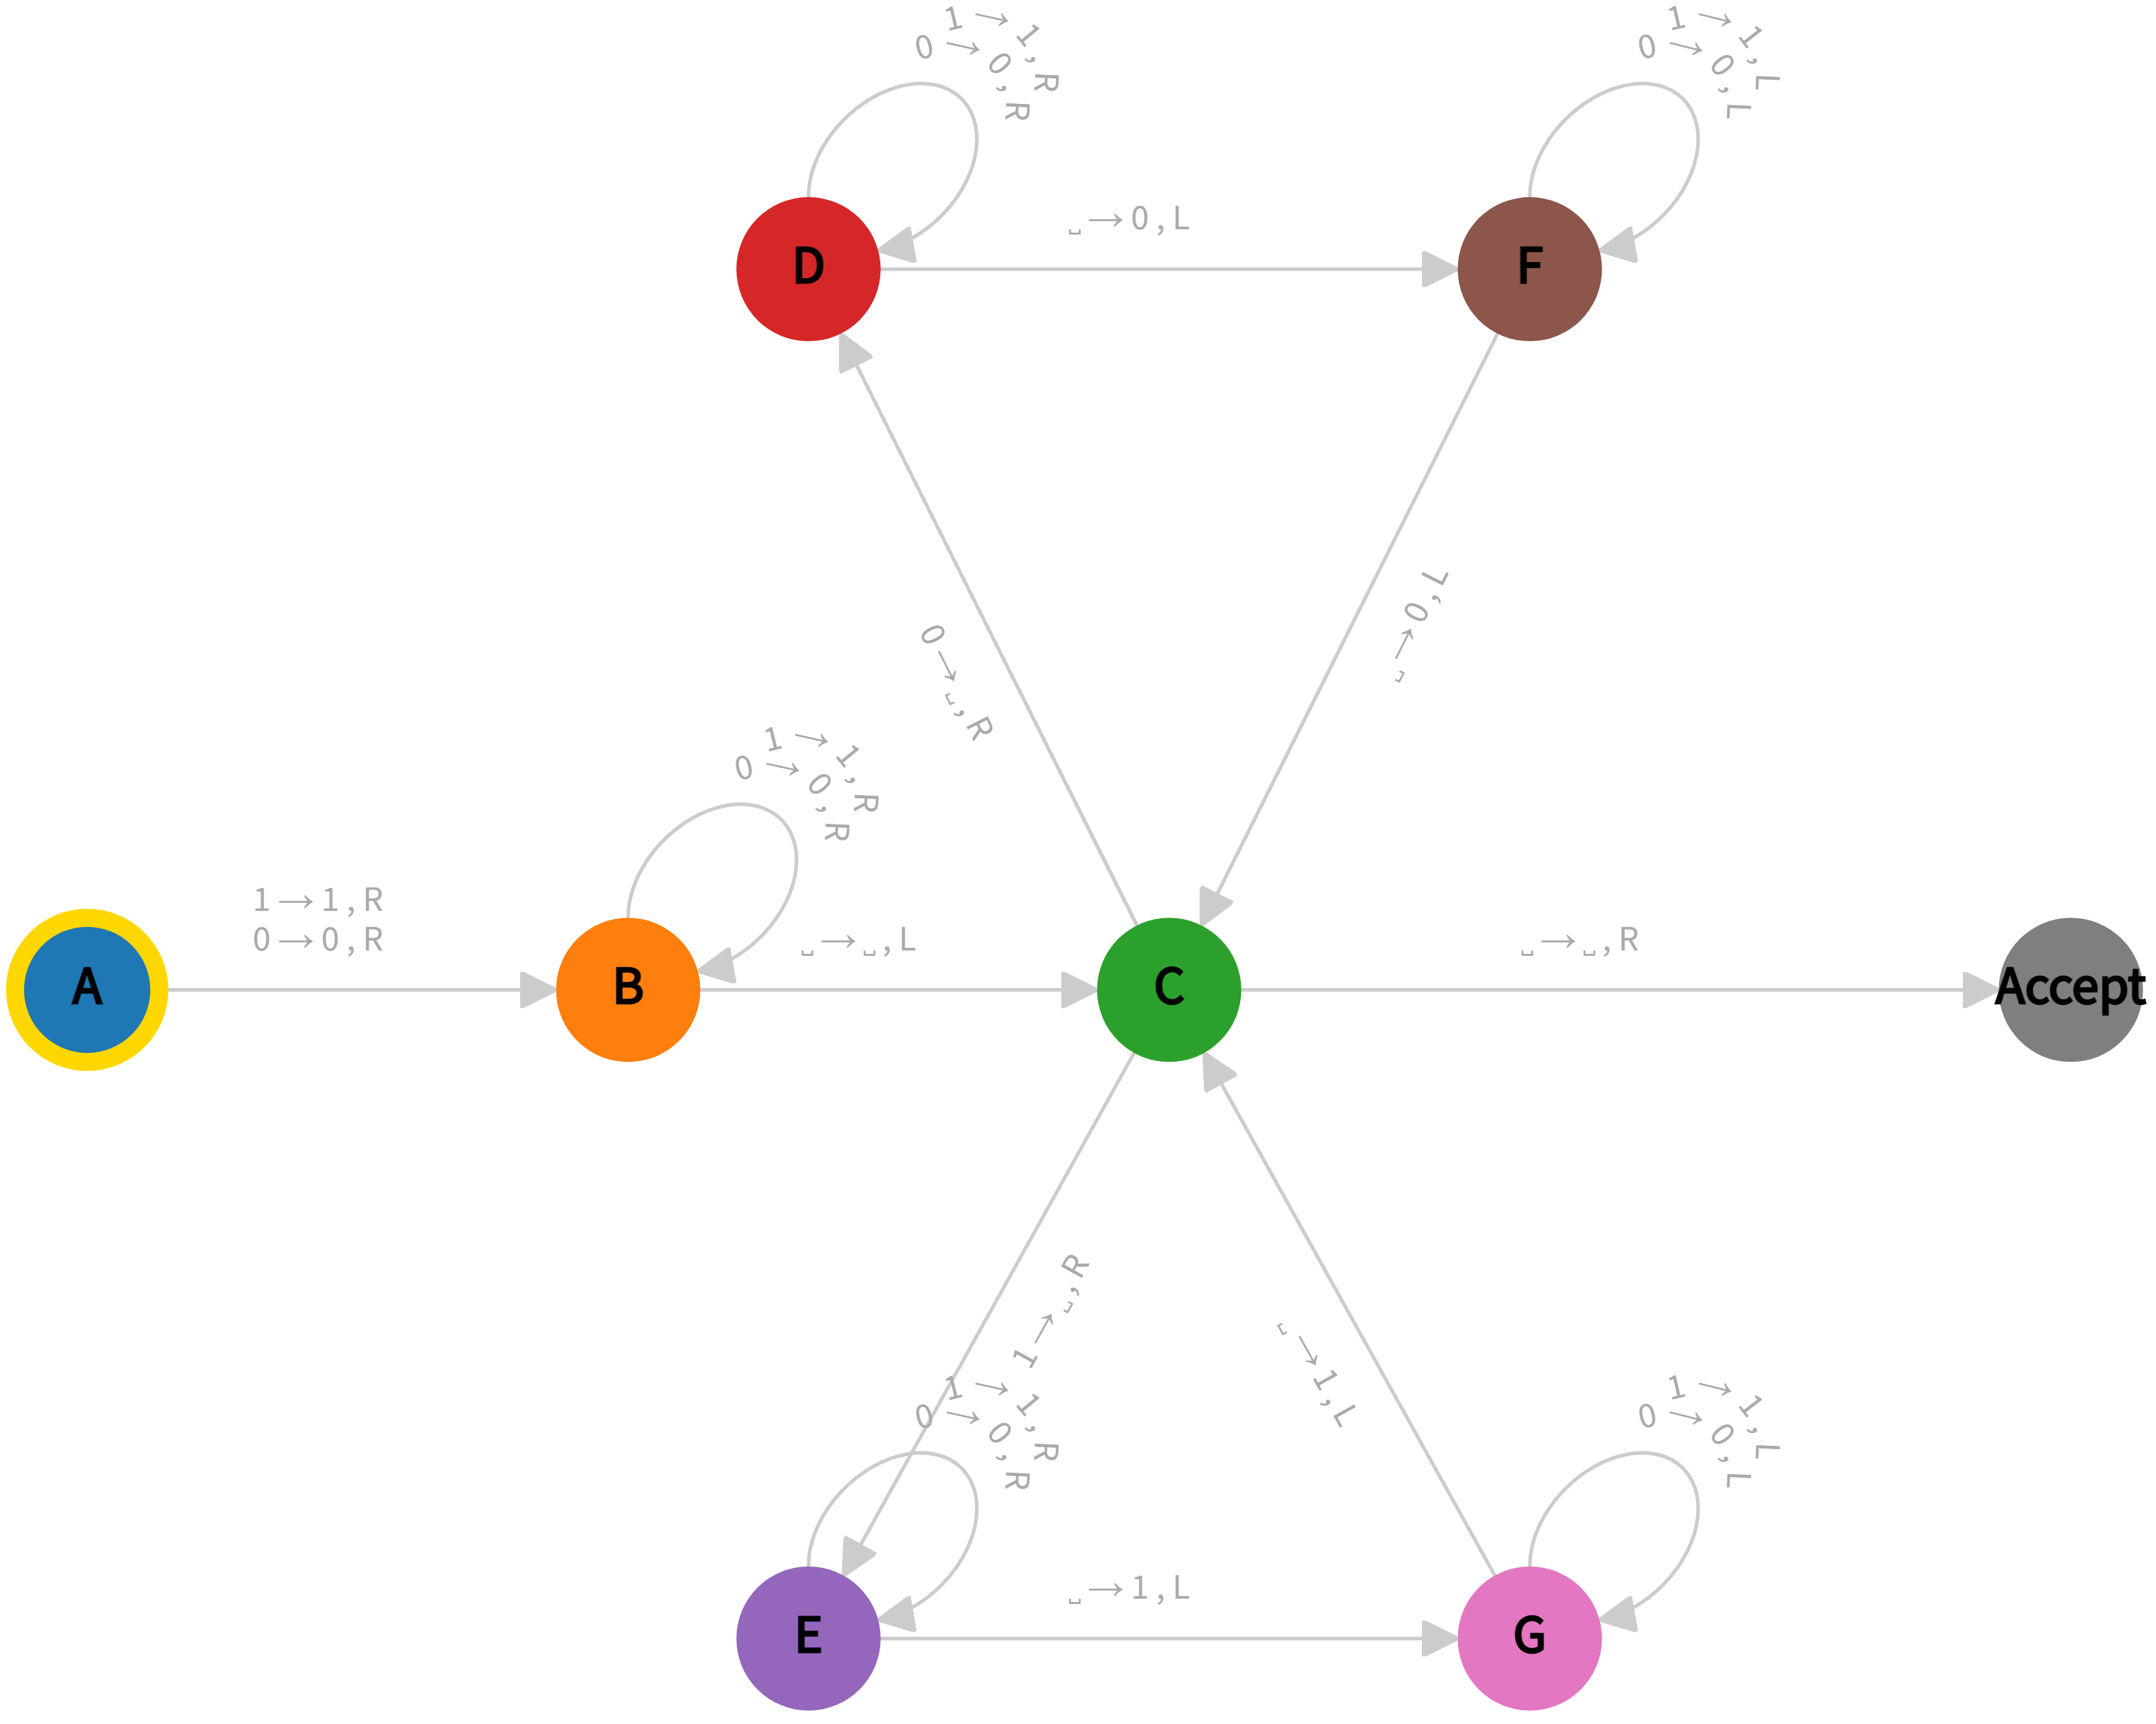
\includegraphics[width=\linewidth]{answers/img/q2-machine.png}
  \caption{\textit{Screenshot of the Turing Machine designed for Q2}}
  \label{fig:q2-machine}
\end{figure}
\vspace*{\fill}

\newpage

\begin{center} \subsection*{Descriptions of States} \end{center}
\label{q2:description-of-states}

\subsubsection*{State: A}
\label{q2-state:initial}

\textit{It is the start state}. If string starts with $\blank$, machine immediately stops in this state. If string starts with $\mathbf{0}$ or $\mathbf{0}$, head is moved to right and state of machine goes to state \hyperref[q2-state:B]{$\mathbf{B}$}.

\subsubsection*{State: B}
\label{q2-state:B}

It scans to the right for the first $\blank$. When $\blank$ is found, head is moved to left and state of machine goes to state \hyperref[q2-state:C]{$\mathbf{C}$}. 

It is used only once to find the last symbol in the string.

\subsubsection*{State: C}
\label{q2-state:C}

It is the state indicating that the symbol below the head needs to be put the end of string; that is, head is on the symbol that will be copied to the end of the string if state of machine is in state \hyperref[q2-state:C]{$\mathbf{C}$}. In this state,
\begin{itemize}
  \item If $\mathbf{0}$ is read, a $\blank$ is temporarily placed and head is moved right and state of machine goes to state \hyperref[q2-state:D]{$\mathbf{D}$} (The upper part of states, as shown in \hyperref[fig:q2-machine]{Figure 8}. This part remembers the symbol was $\mathbf{0}$).
  \item If $\mathbf{1}$ is read, a $\blank$ is temporarily placed and head is moved right and state of machine goes to state \hyperref[q2-state:E]{$\mathbf{E}$} (The lower part of states, as shown in \hyperref[fig:q2-machine]{Figure 8}. This part remembers the symbol was $\mathbf{1}$).
  \item If $\blank$ is read, it means that computing is done without any error or crash. State of the machine goes to state \hyperref[q2-state:Accept]{$\mathbf{Accept}$}
\end{itemize}

\subsubsection*{State: D}
\label{q2-state:D}

It scans to the right for the first $\blank$. The important part is that it knows (symbol that will be copied was $\mathbf{0}$) symbol will be written is $\mathbf{0}$. When $\blank$ is found,
\begin{itemize}
  \item $\mathbf{0}$ is placed,
  \item head is moved left, and
  \item state of the machine goes to state \hyperref[q2-state:F]{$\mathbf{F}$}.
\end{itemize}

\subsubsection*{State: F}
\label{q2-state:F}

It scans to the left for the $\blank$ that is placed temporarily. The important part is that it knows (copied symbol was $\mathbf{0}$) symbol will be written is $\mathbf{0}$. When $\blank$ is found,
\begin{itemize}
  \item $\mathbf{0}$ is reinserted to its old place,
  \item head is moved left (next is symbol that will be copied or a $\blank$), and
  \item state of the machine goes to state \hyperref[q2-state:C]{$\mathbf{C}$}.
\end{itemize}

\subsubsection*{State: E}
\label{q2-state:E}

It scans to the right for the first $\blank$. The important part is that it knows (symbol that will be copied was $\mathbf{1}$) symbol will be written is $\mathbf{1}$. When $\blank$ is found,
\begin{itemize}
  \item $\mathbf{1}$ is placed,
  \item head is moved left, and
  \item state of the machine goes to state \hyperref[q2-state:G]{$\mathbf{G}$}.
\end{itemize}

\subsubsection*{State: G}
\label{q2-state:G}

It scans to the left for the $\blank$ that is placed temporarily. The important part is that it knows (copied symbol was $\mathbf{1}$) symbol will be written is $\mathbf{1}$. When $\blank$ is found,
\begin{itemize}
  \item $\mathbf{1}$ is reinserted to its old place,
  \item head is moved left (next is symbol that will be copied or a $\blank$), and
  \item state of the machine goes to state \hyperref[q2-state:C]{$\mathbf{C}$}.
\end{itemize}

\subsubsection*{State: Accept}
\label{q2-state:Accept}

\textit{It is state indicating that computing is done without any error or crash}. Therefore, the machine stops, successfully.


\newpage

\begin{center} \subsection*{Input Samples} \end{center}
\label{q2:input-samples}
\vspace*{\fill}

\subsubsection*{Input: 1011}
\label{q2-1011}

\begin{figure}[ht]
  \centering
  \begin{minipage}{.49\linewidth}
    \centering
    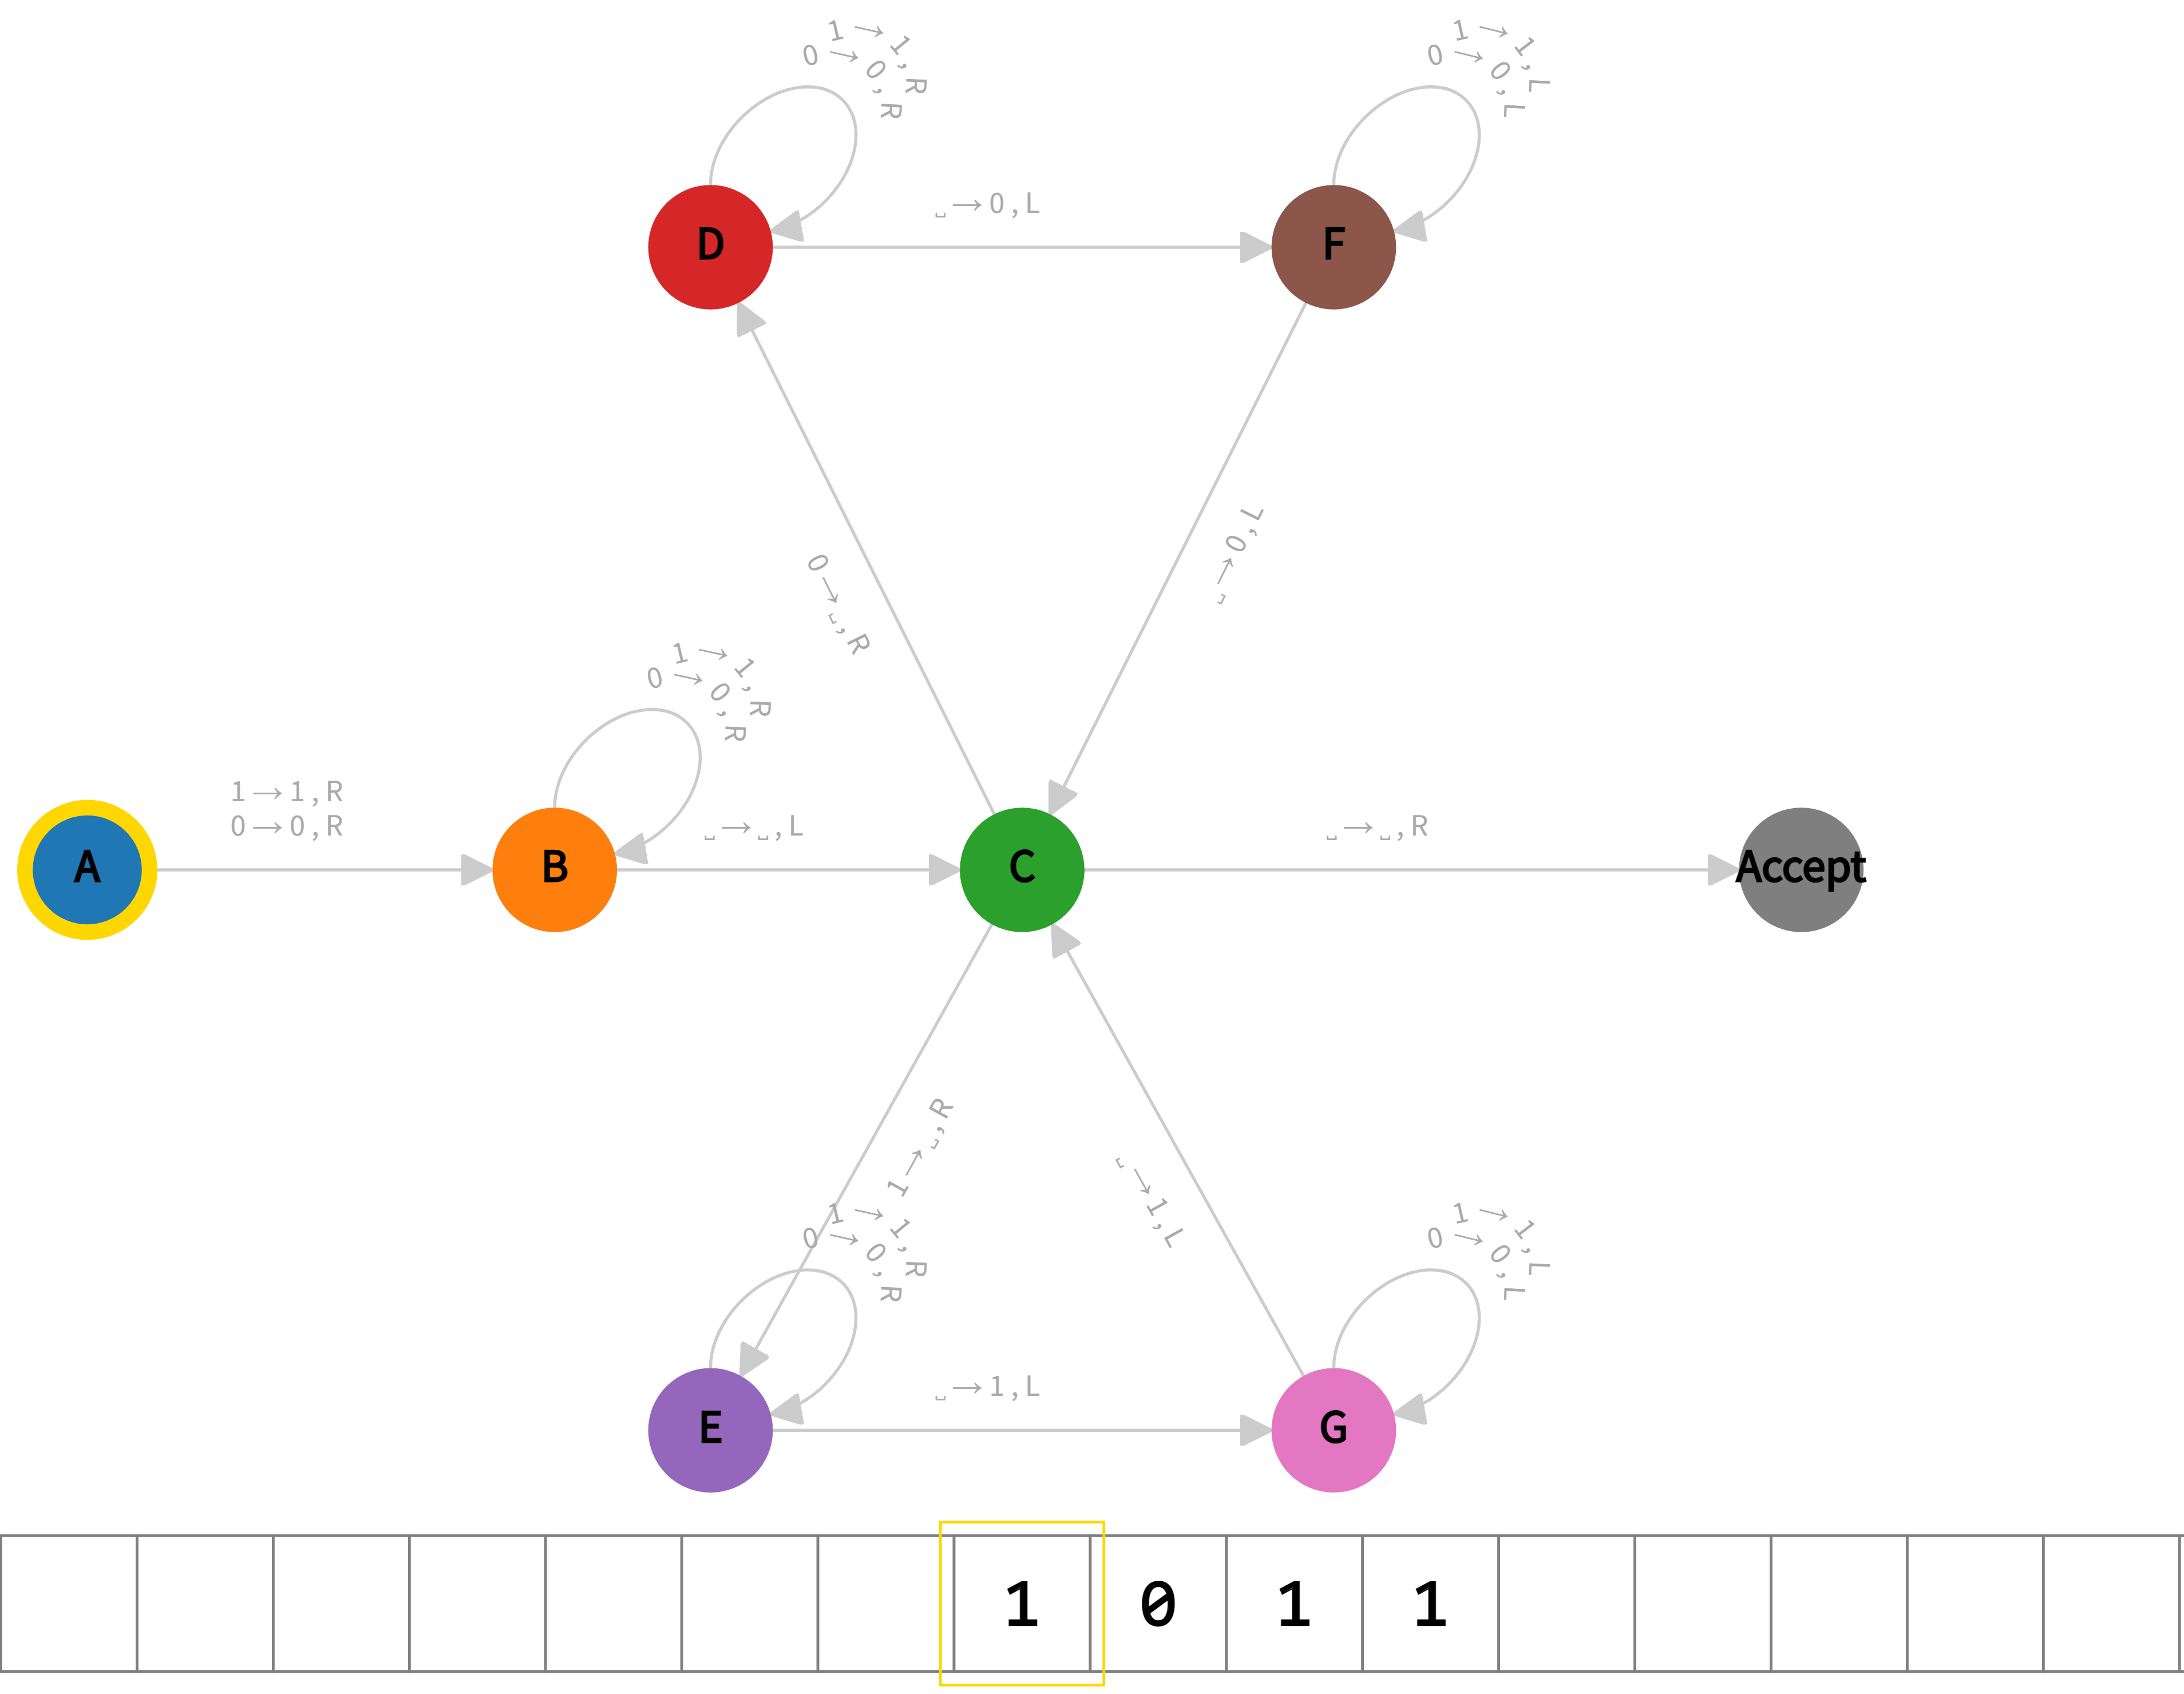
\includegraphics[width=\linewidth]{answers/img/q2-1011-initial.png}
    \caption*{Figure (a): Initial State for $\mathbf{1011}$}
    \label{fig:1011-initial}
  \end{minipage}
  \begin{minipage}{.49\linewidth}
    \centering
    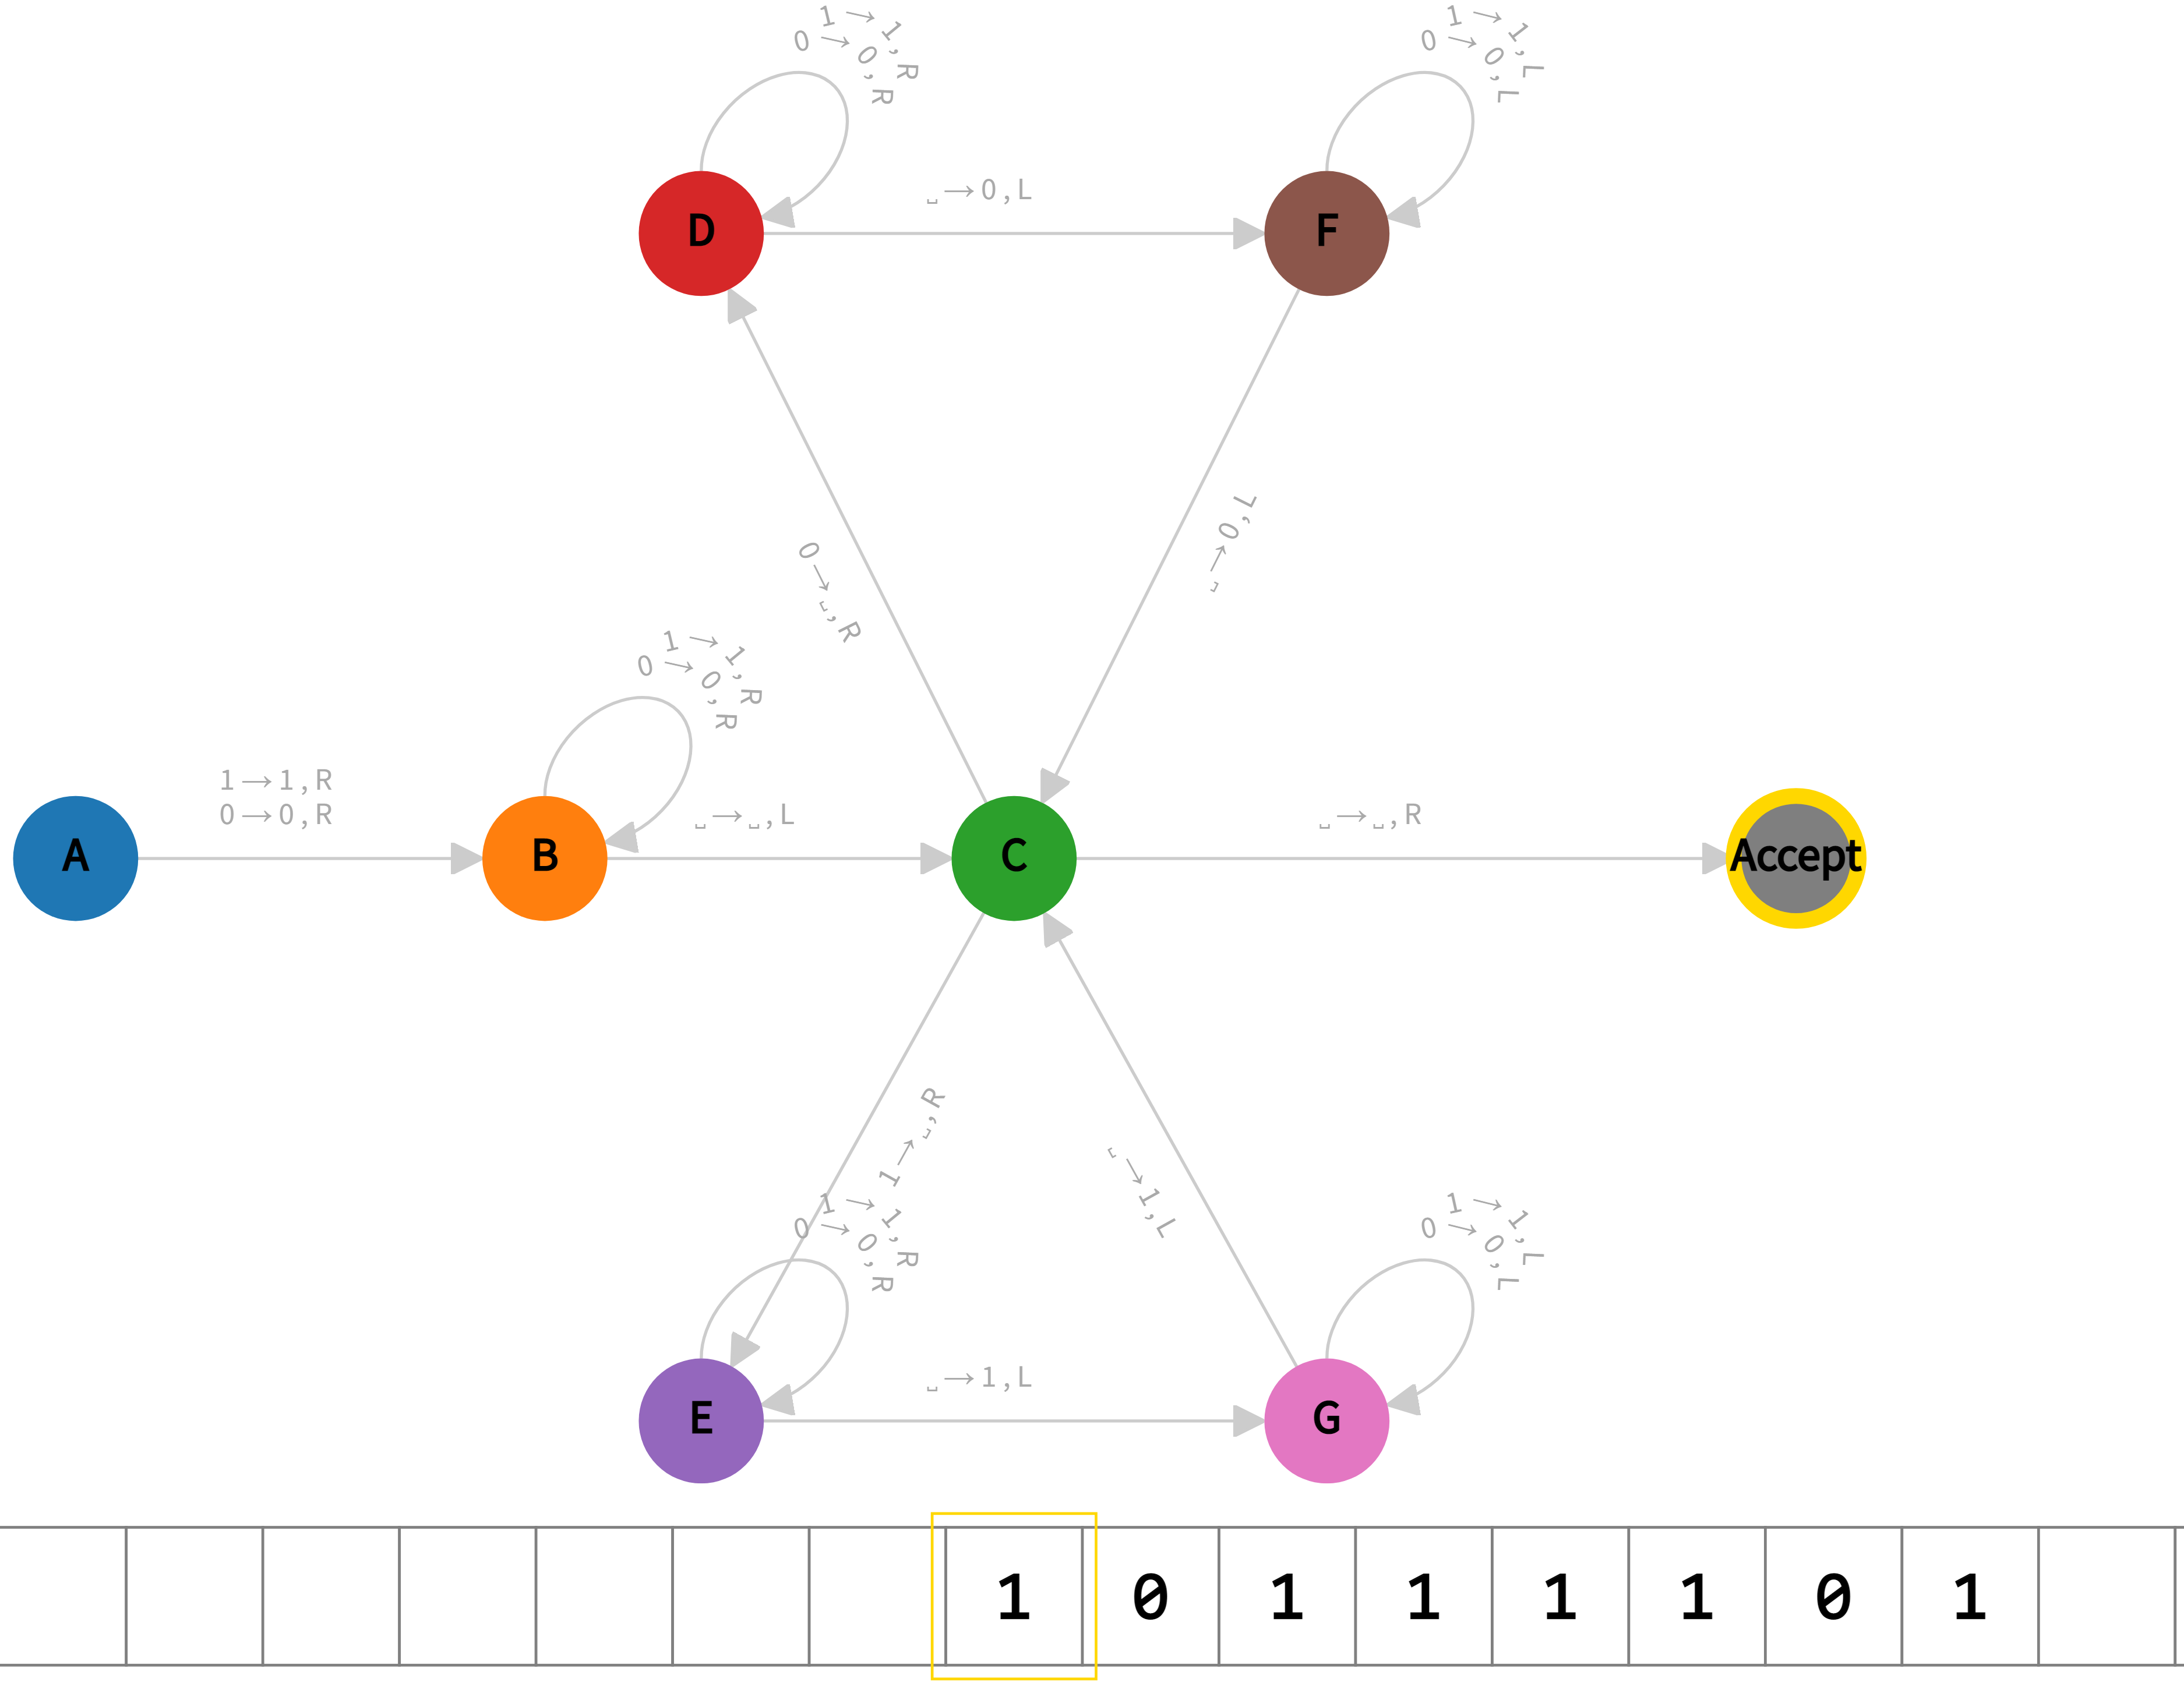
\includegraphics[width=\linewidth]{answers/img/q2-1011-end.png}
    \caption*{Figure (b): End State for $\mathbf{1011}$}
    \label{fig:1011-end}
  \end{minipage}
  \caption{States for $\mathbf{1011}$}
  \label{fig:in-1011}
\end{figure}

\subsubsection*{Input: 1110}
\label{q2-1110}

\begin{figure}[ht]
  \centering
  \begin{minipage}{.49\linewidth}
    \centering
    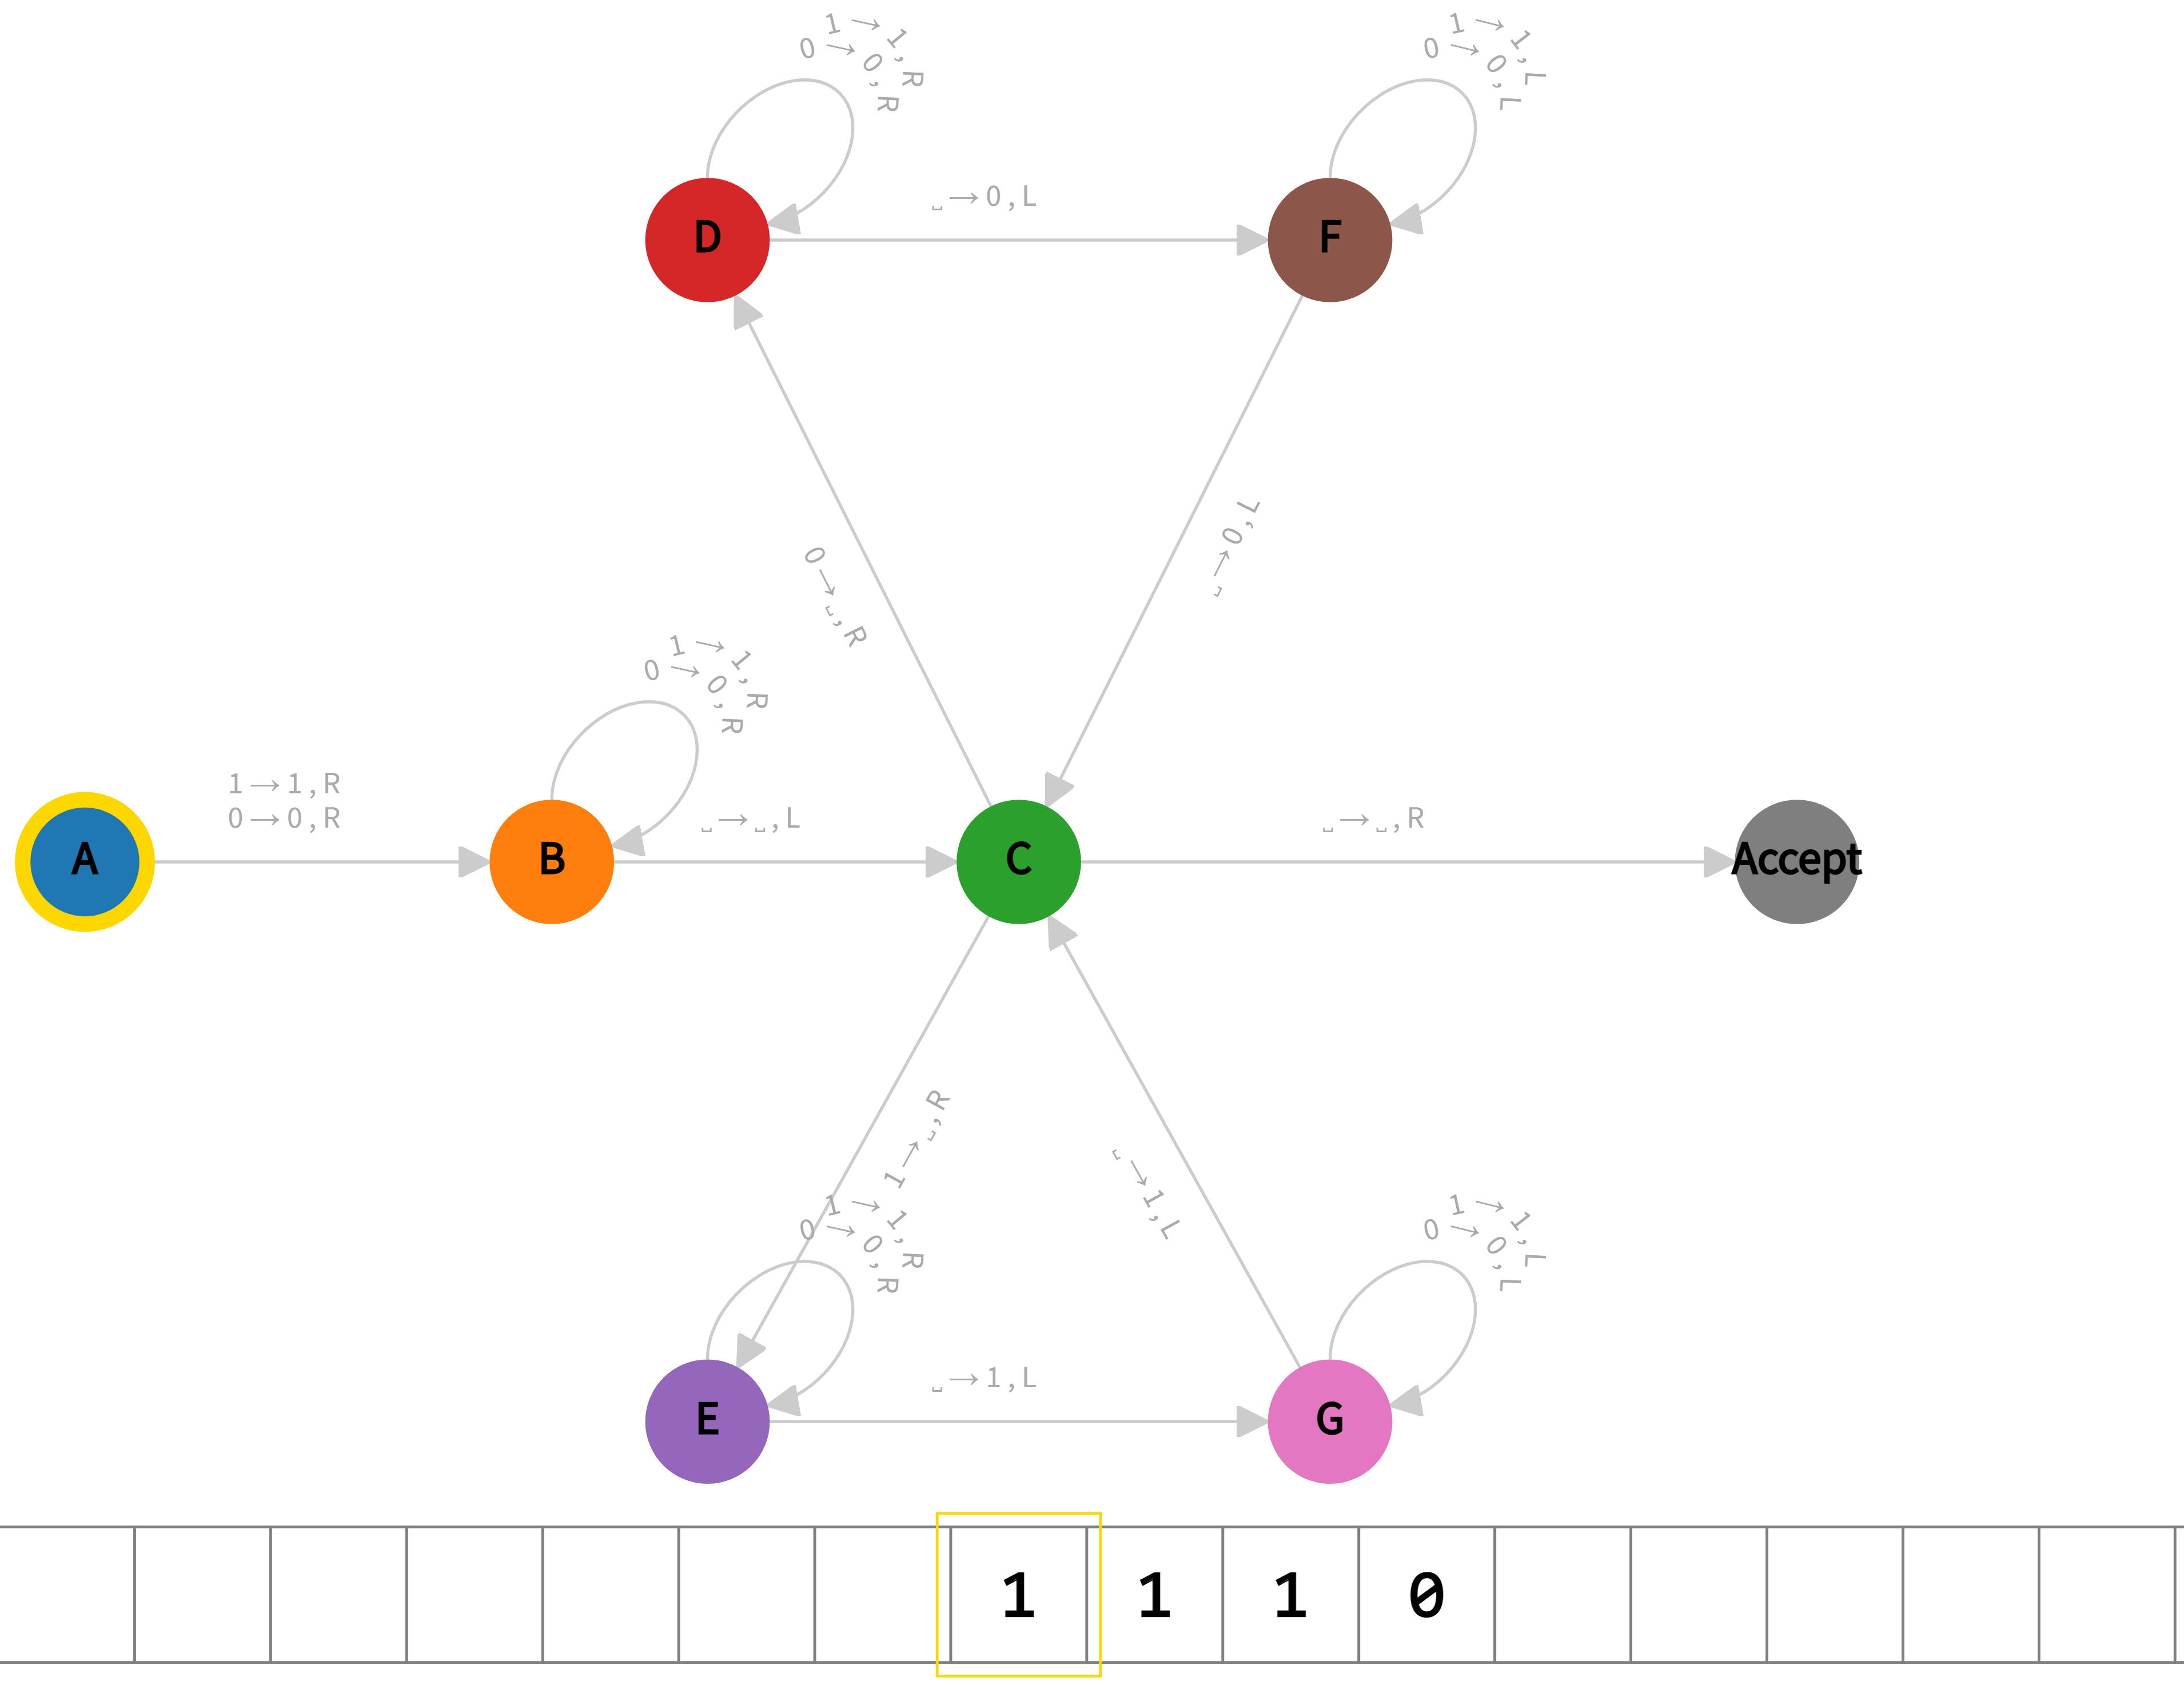
\includegraphics[width=\linewidth]{answers/img/q2-1110-initial.png}
    \caption*{Figure (a): Initial State for $\mathbf{1110}$}
    \label{fig:1110-initial}
  \end{minipage}
  \begin{minipage}{.49\linewidth}
    \centering
    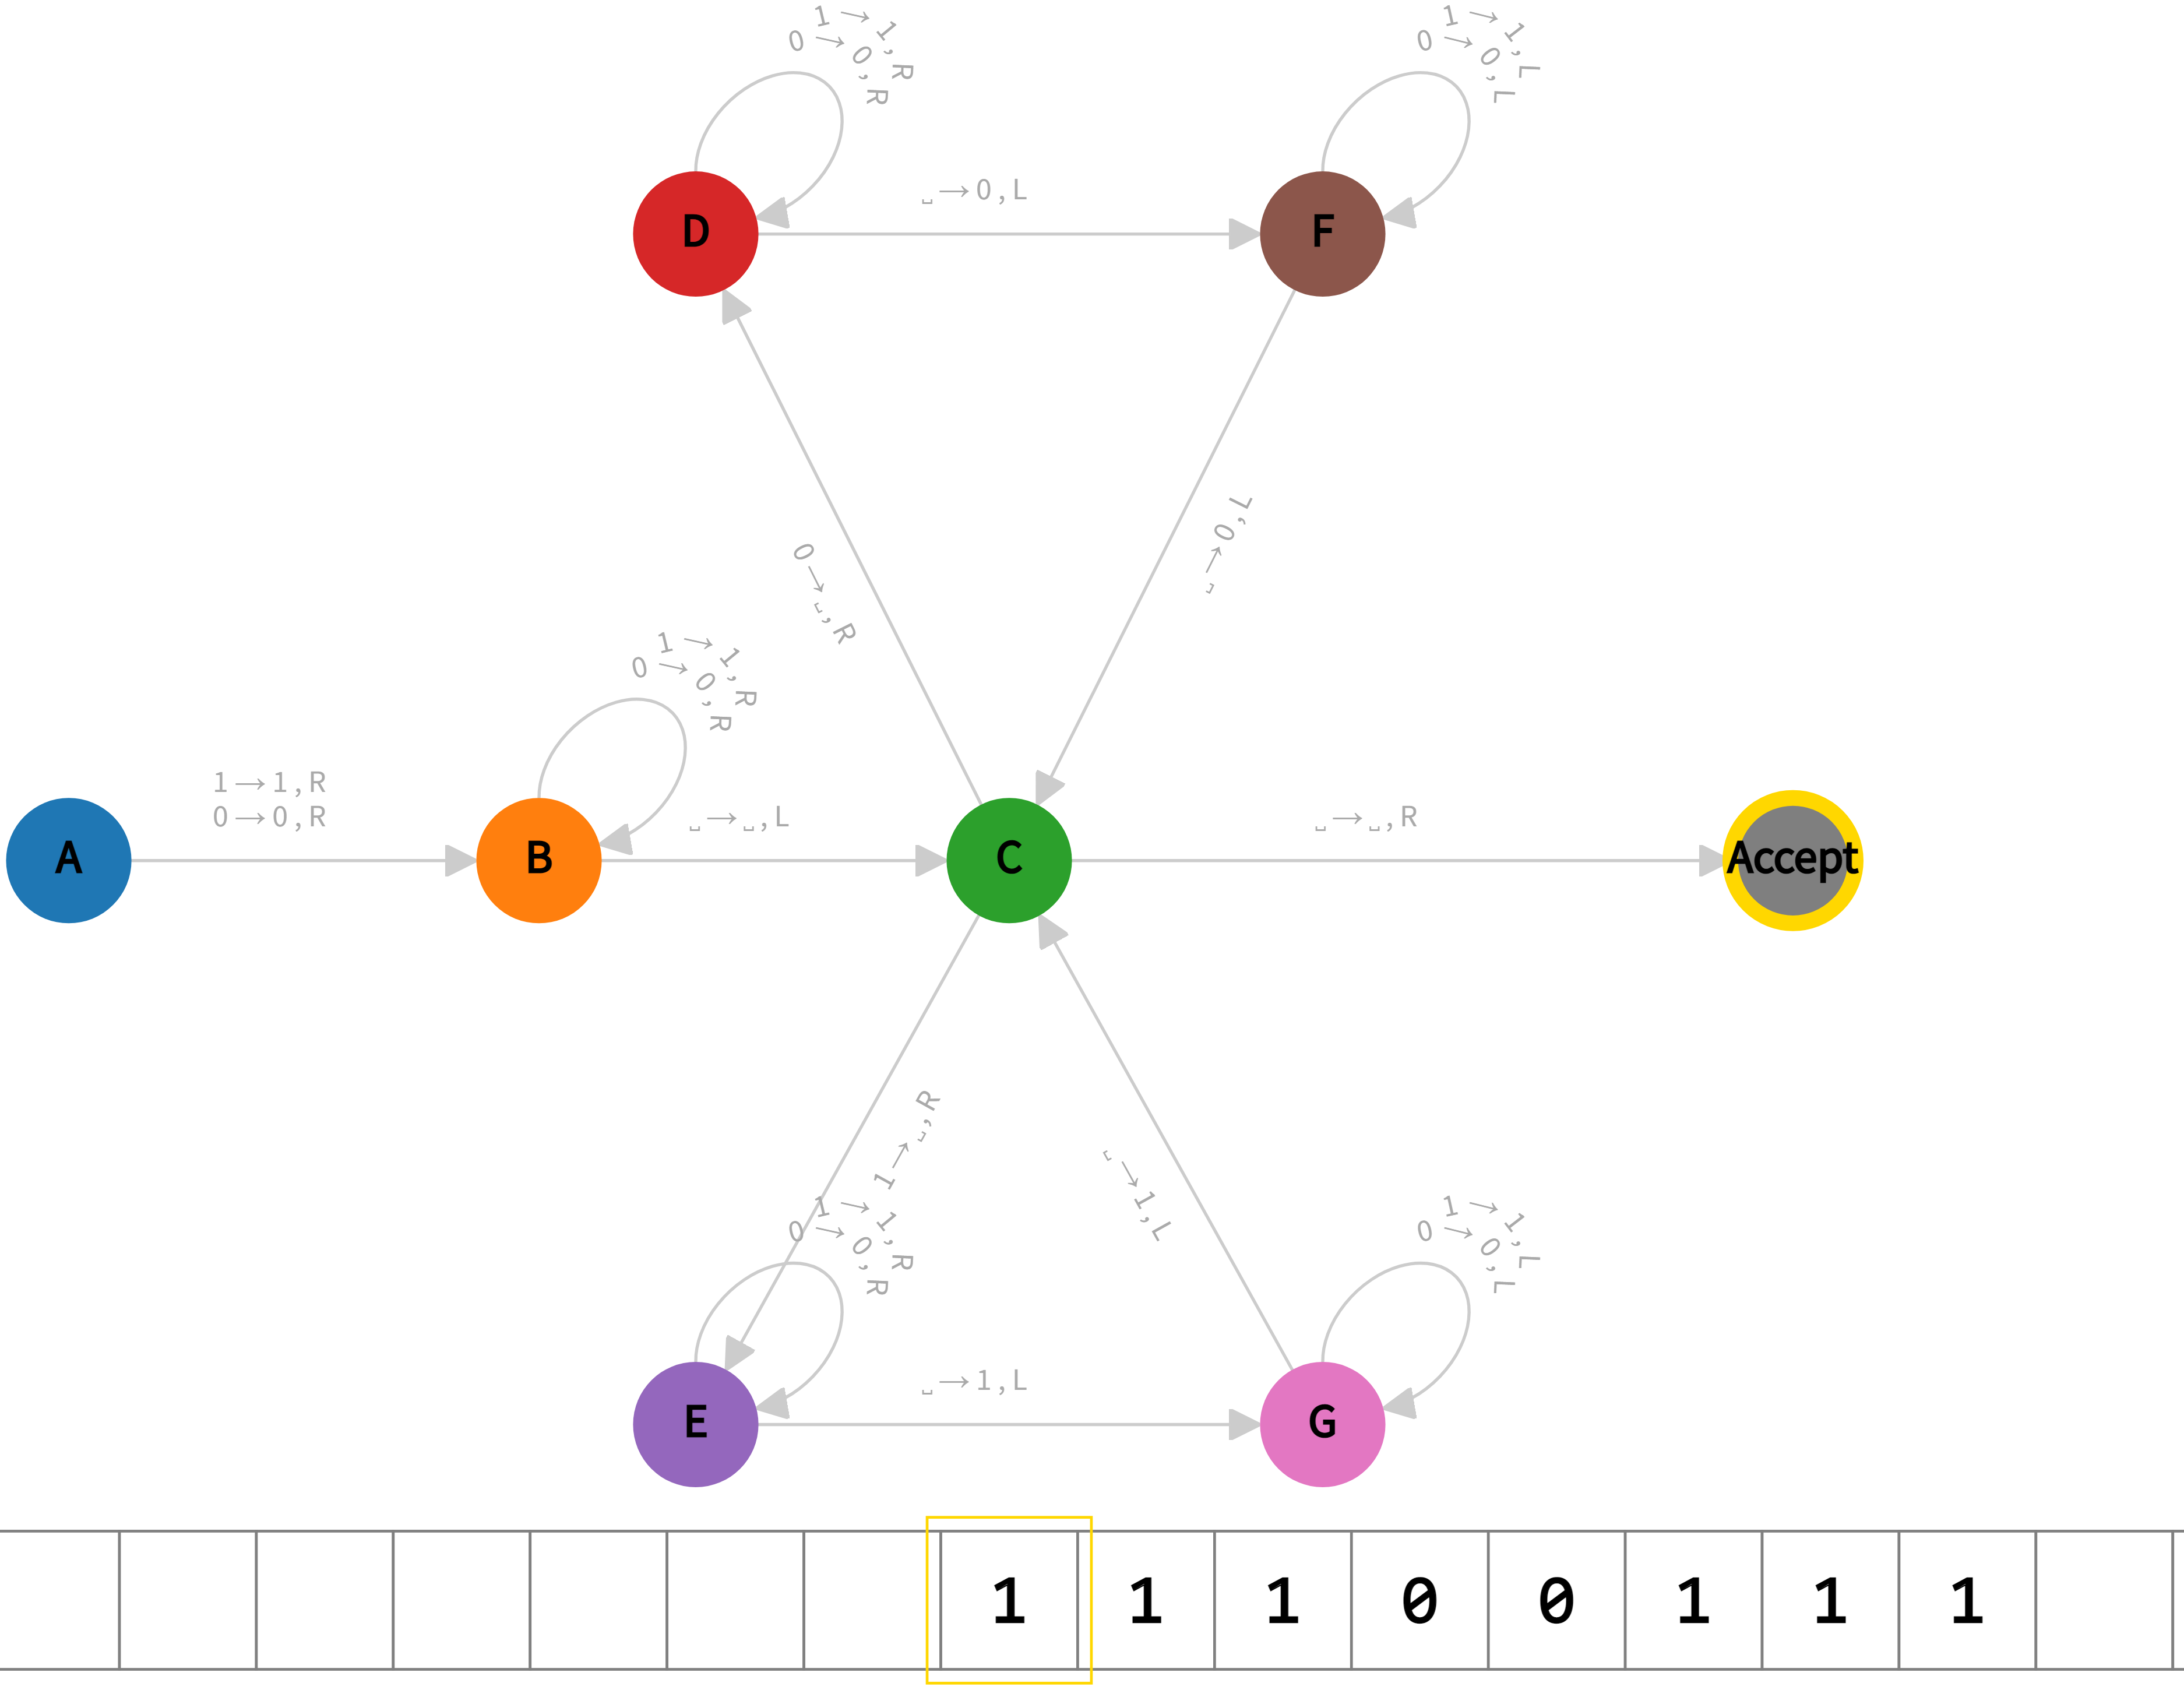
\includegraphics[width=\linewidth]{answers/img/q2-1110-end.png}
    \caption*{Figure (b): End State for $\mathbf{1110}$}
    \label{fig:1110-end}
  \end{minipage}
  \caption{States for $\mathbf{1110}$}
  \label{fig:in-1110}
\end{figure}

\vspace*{\fill}

\newpage

\vspace*{\fill}

\subsubsection*{Input: 0101}
\label{q2-0101}

\begin{figure}[ht]
  \centering
  \begin{minipage}{.49\linewidth}
    \centering
    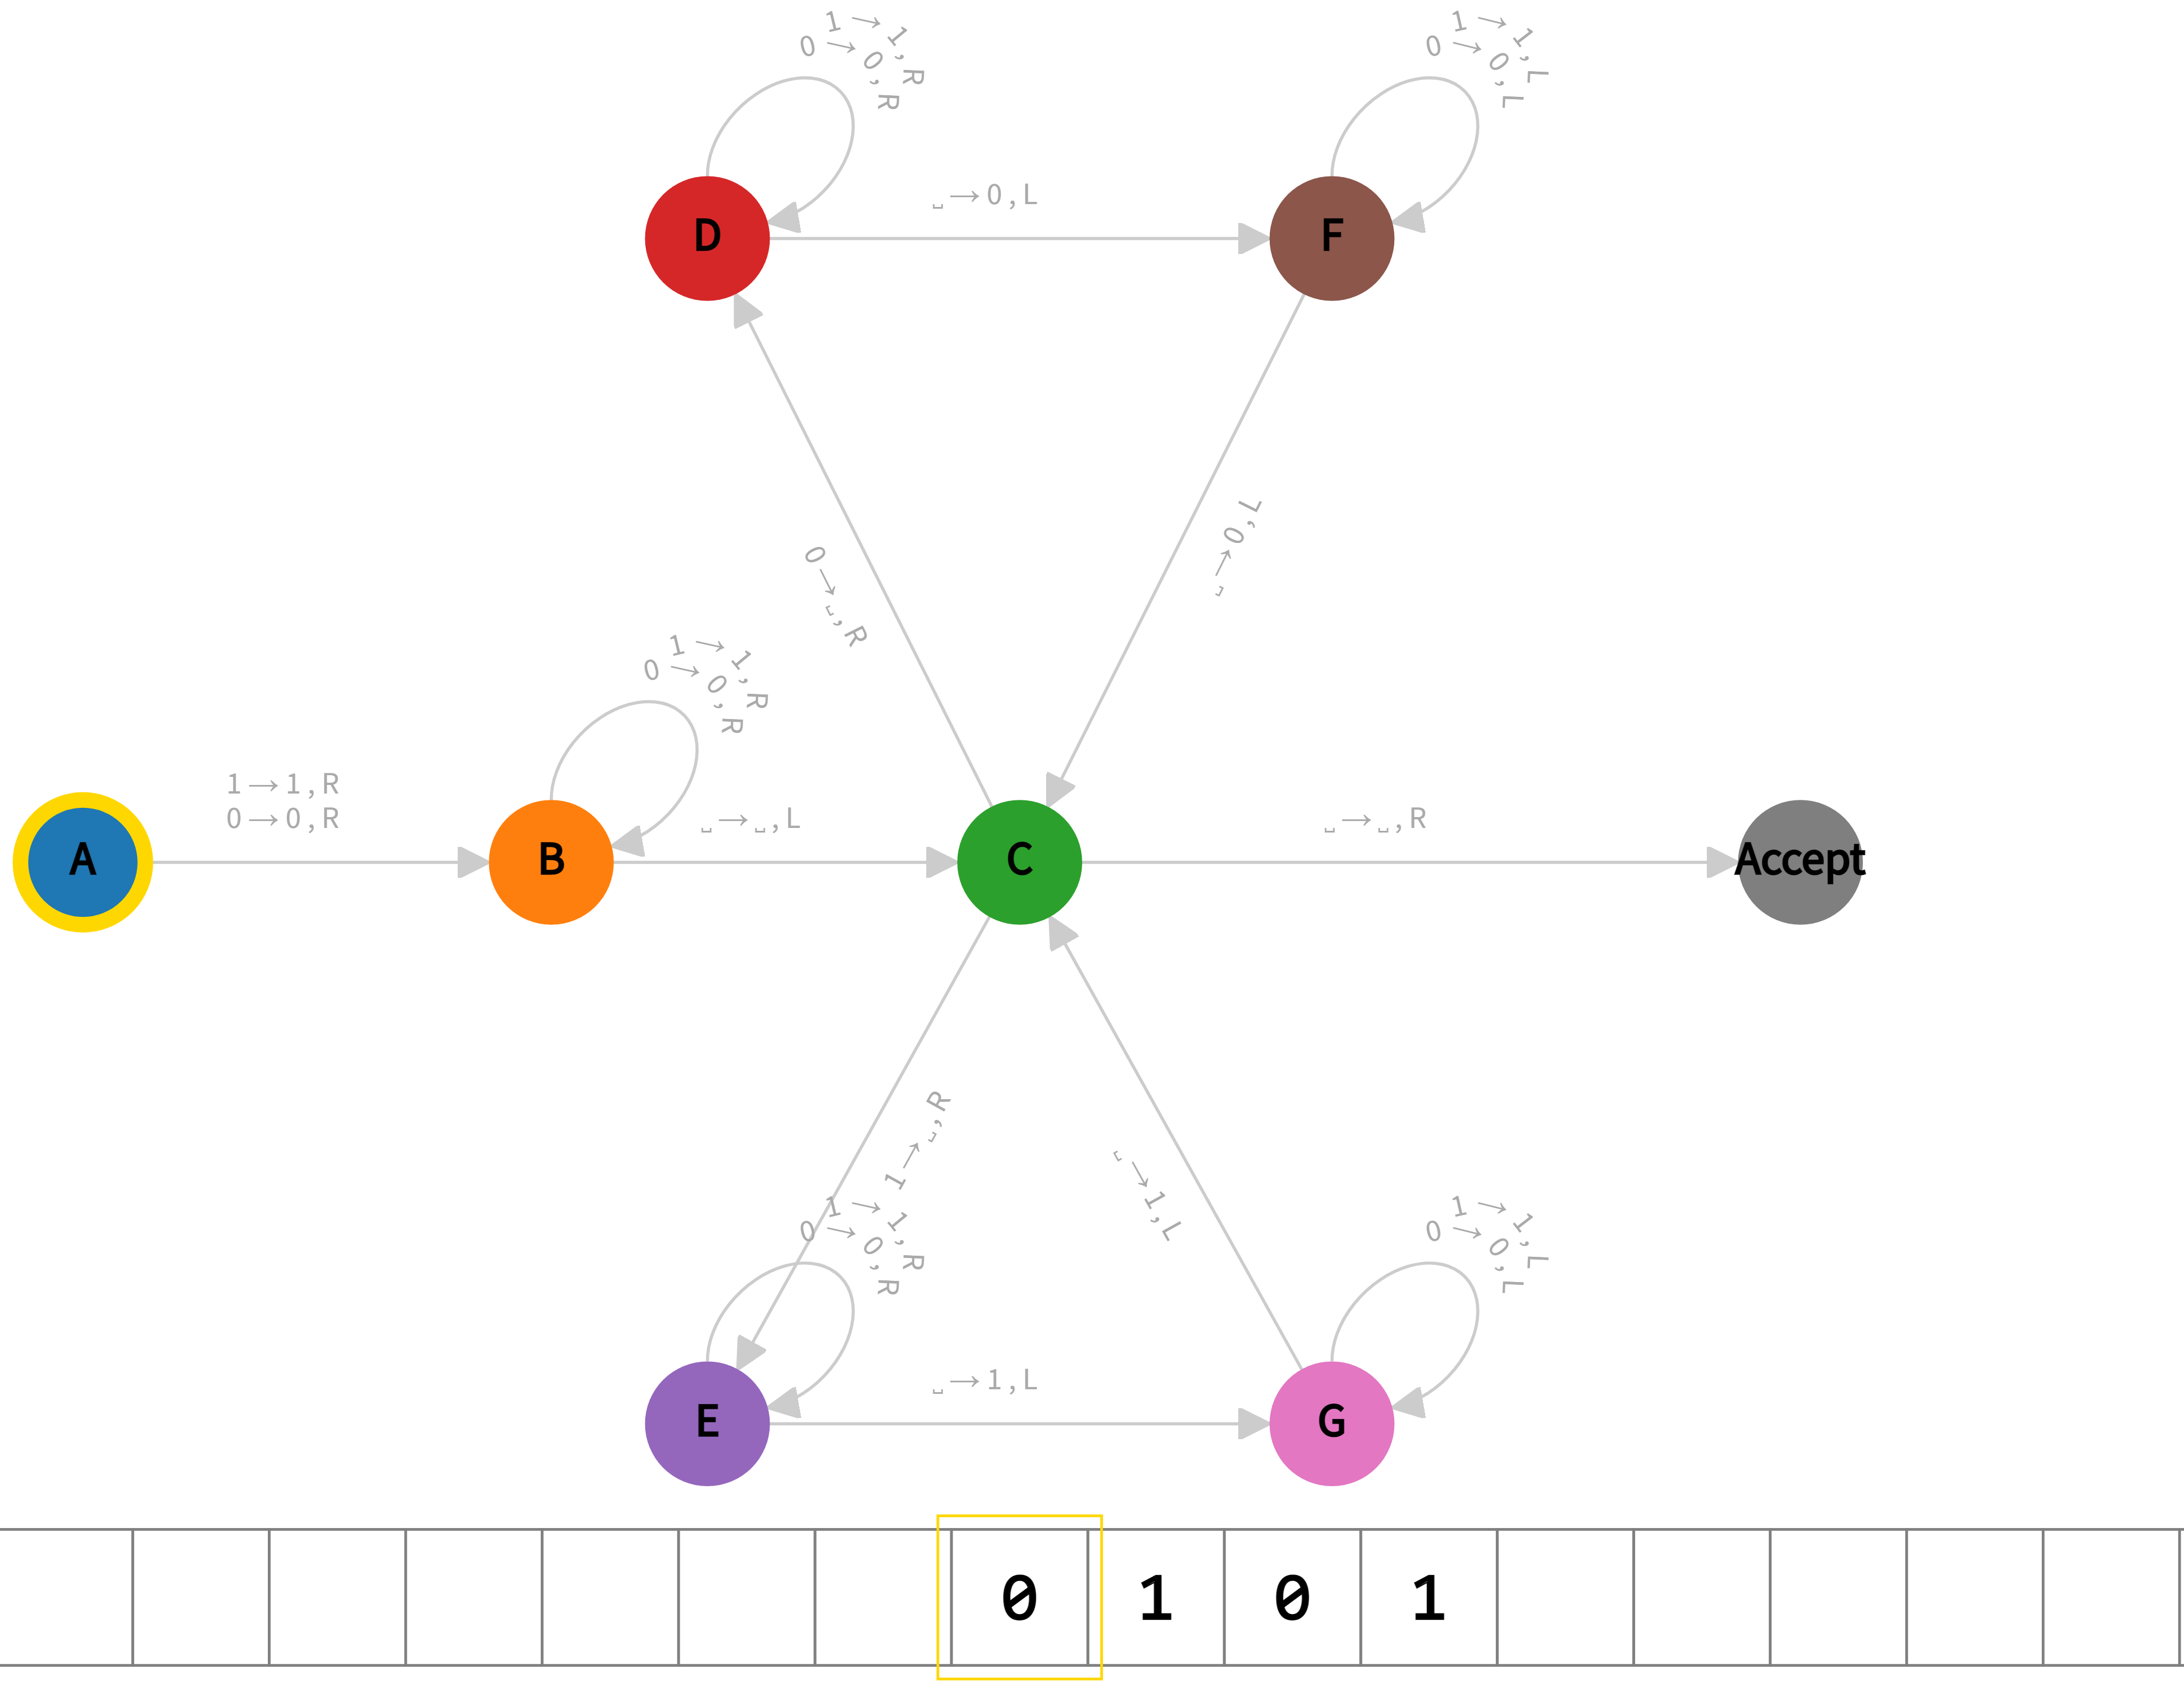
\includegraphics[width=\linewidth]{answers/img/q2-0101-initial.png}
    \caption*{Figure (a): Initial State for $\mathbf{0101}$}
    \label{fig:0101-initial}
  \end{minipage}
  \begin{minipage}{.49\linewidth}
    \centering
    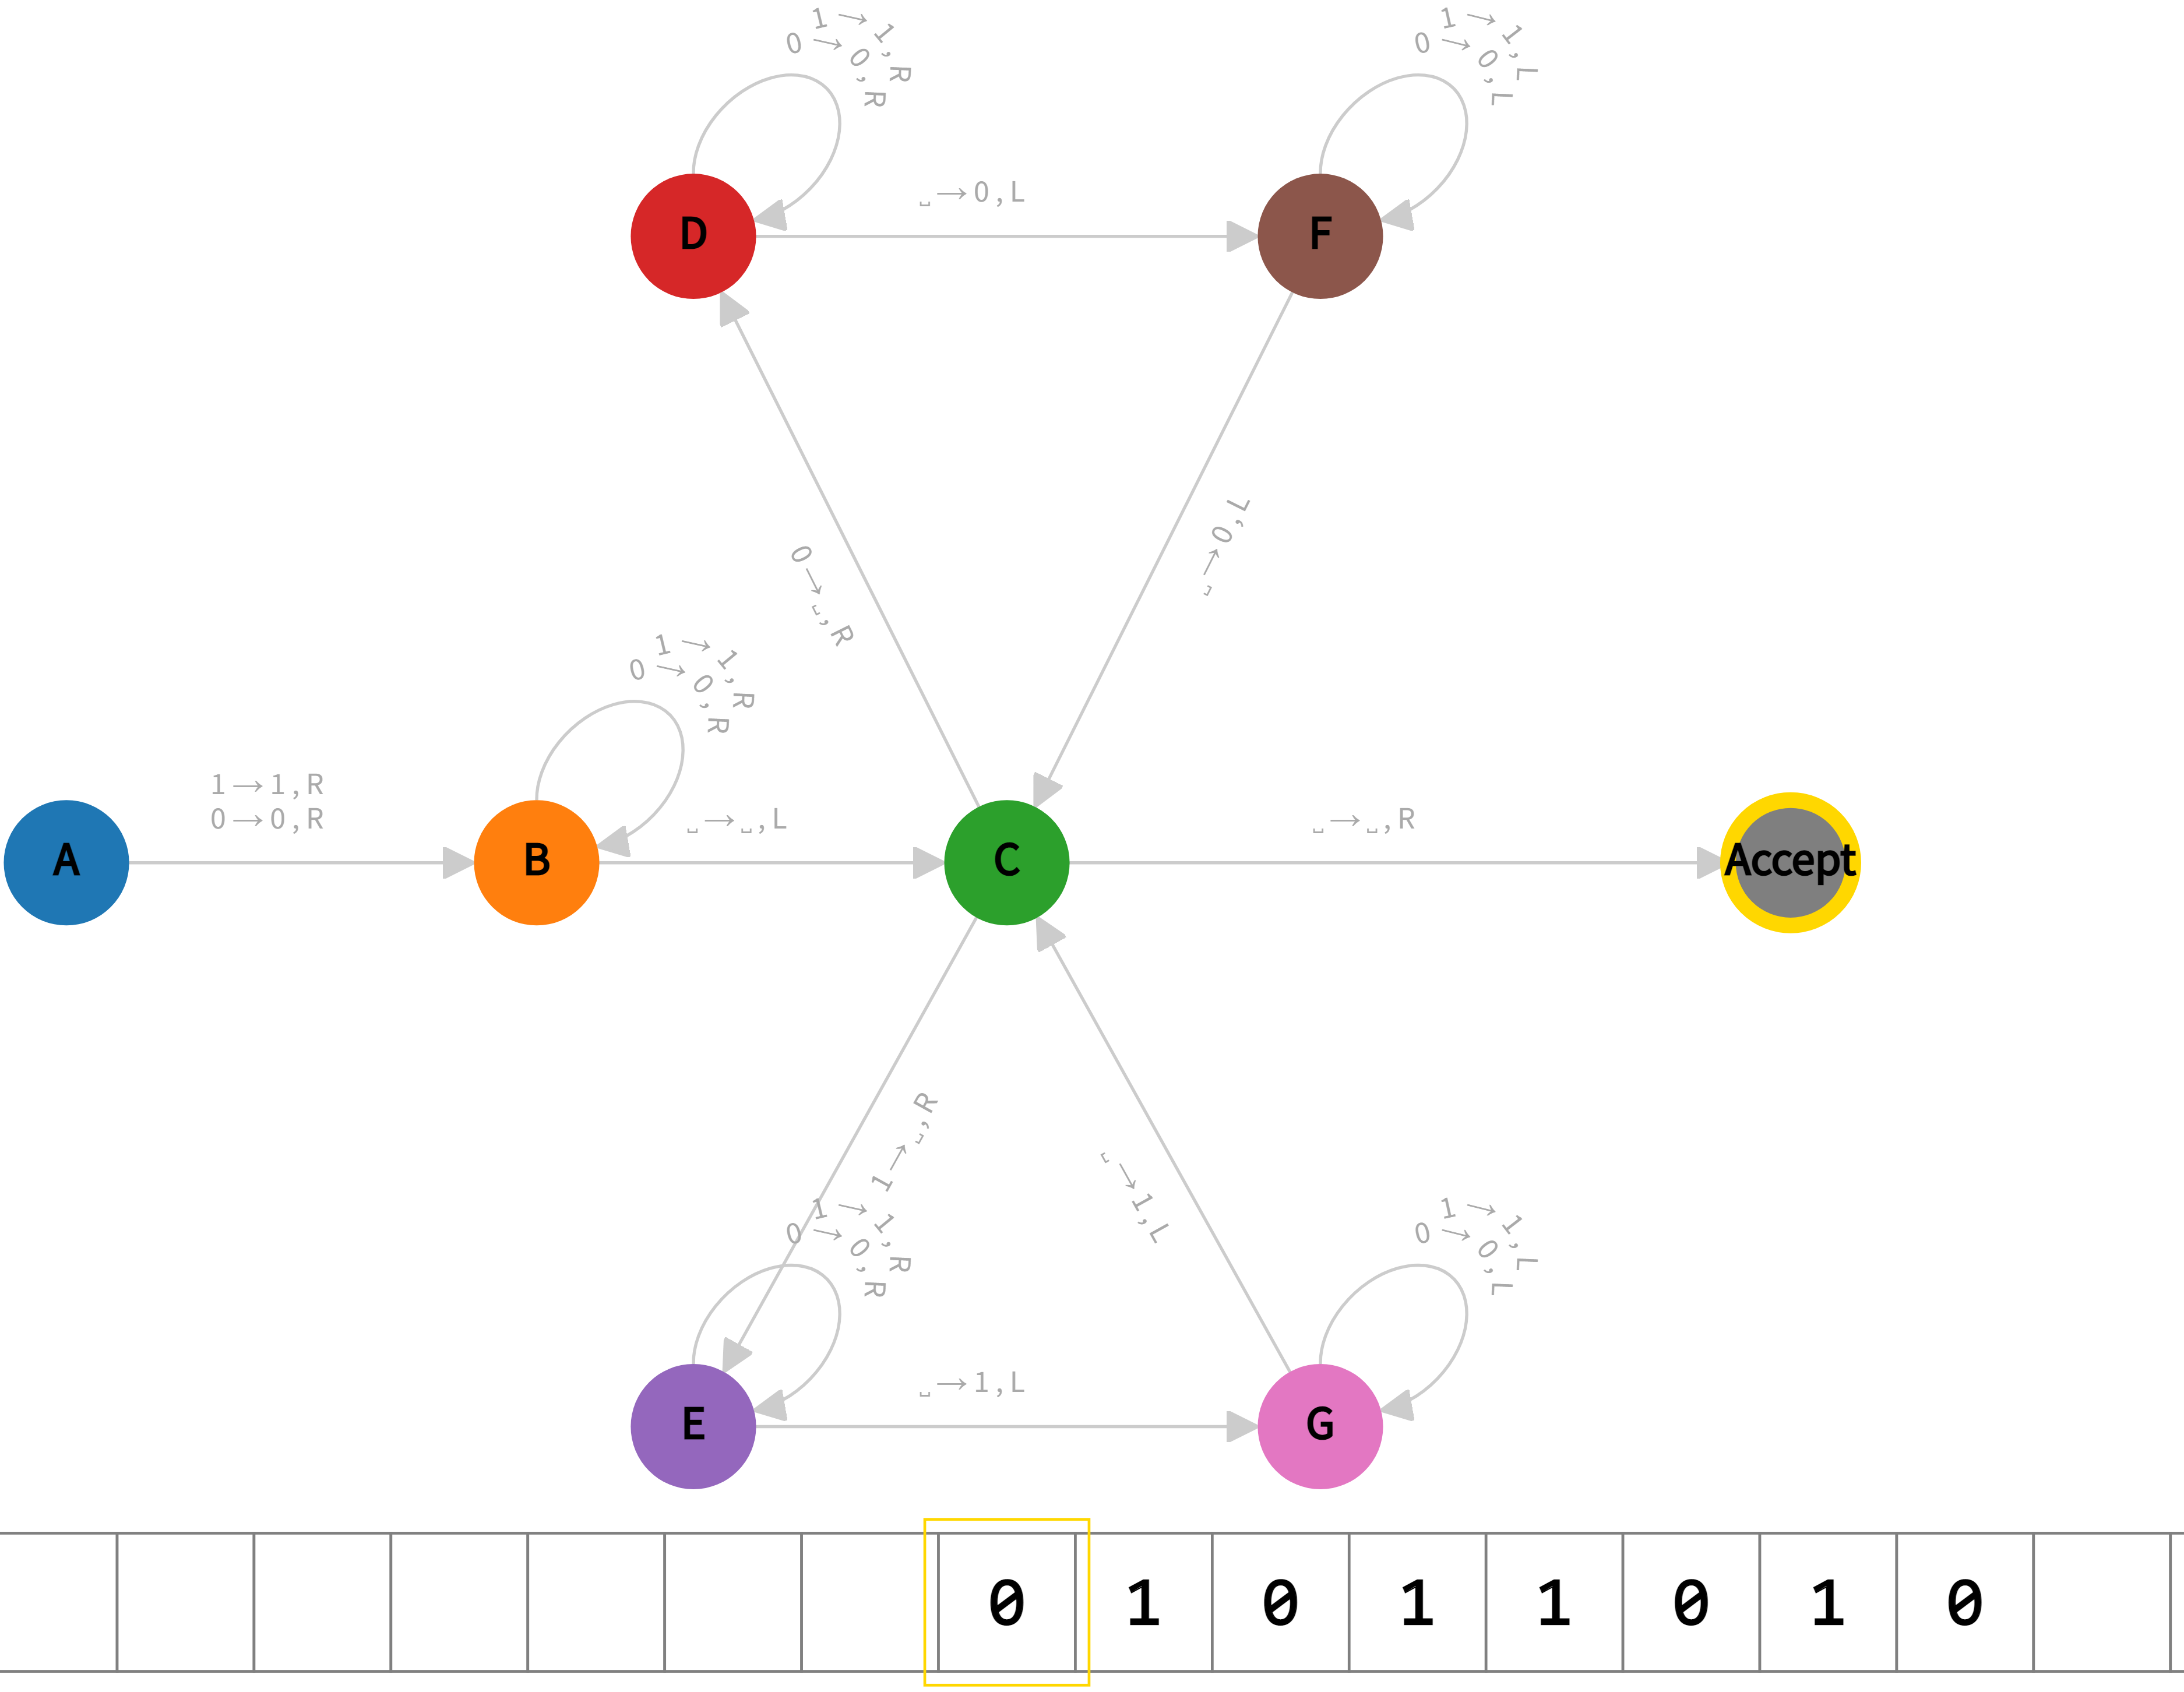
\includegraphics[width=\linewidth]{answers/img/q2-0101-end.png}
    \caption*{Figure (b): End State for $\mathbf{0101}$}
    \label{fig:0101-end}
  \end{minipage}
  \caption{States for $\mathbf{0101}$}
  \label{fig:in-0101}
\end{figure}

\subsubsection*{Input: 1010}
\label{q2-1010}

\begin{figure}[ht]
  \centering
  \begin{minipage}{.49\linewidth}
    \centering
    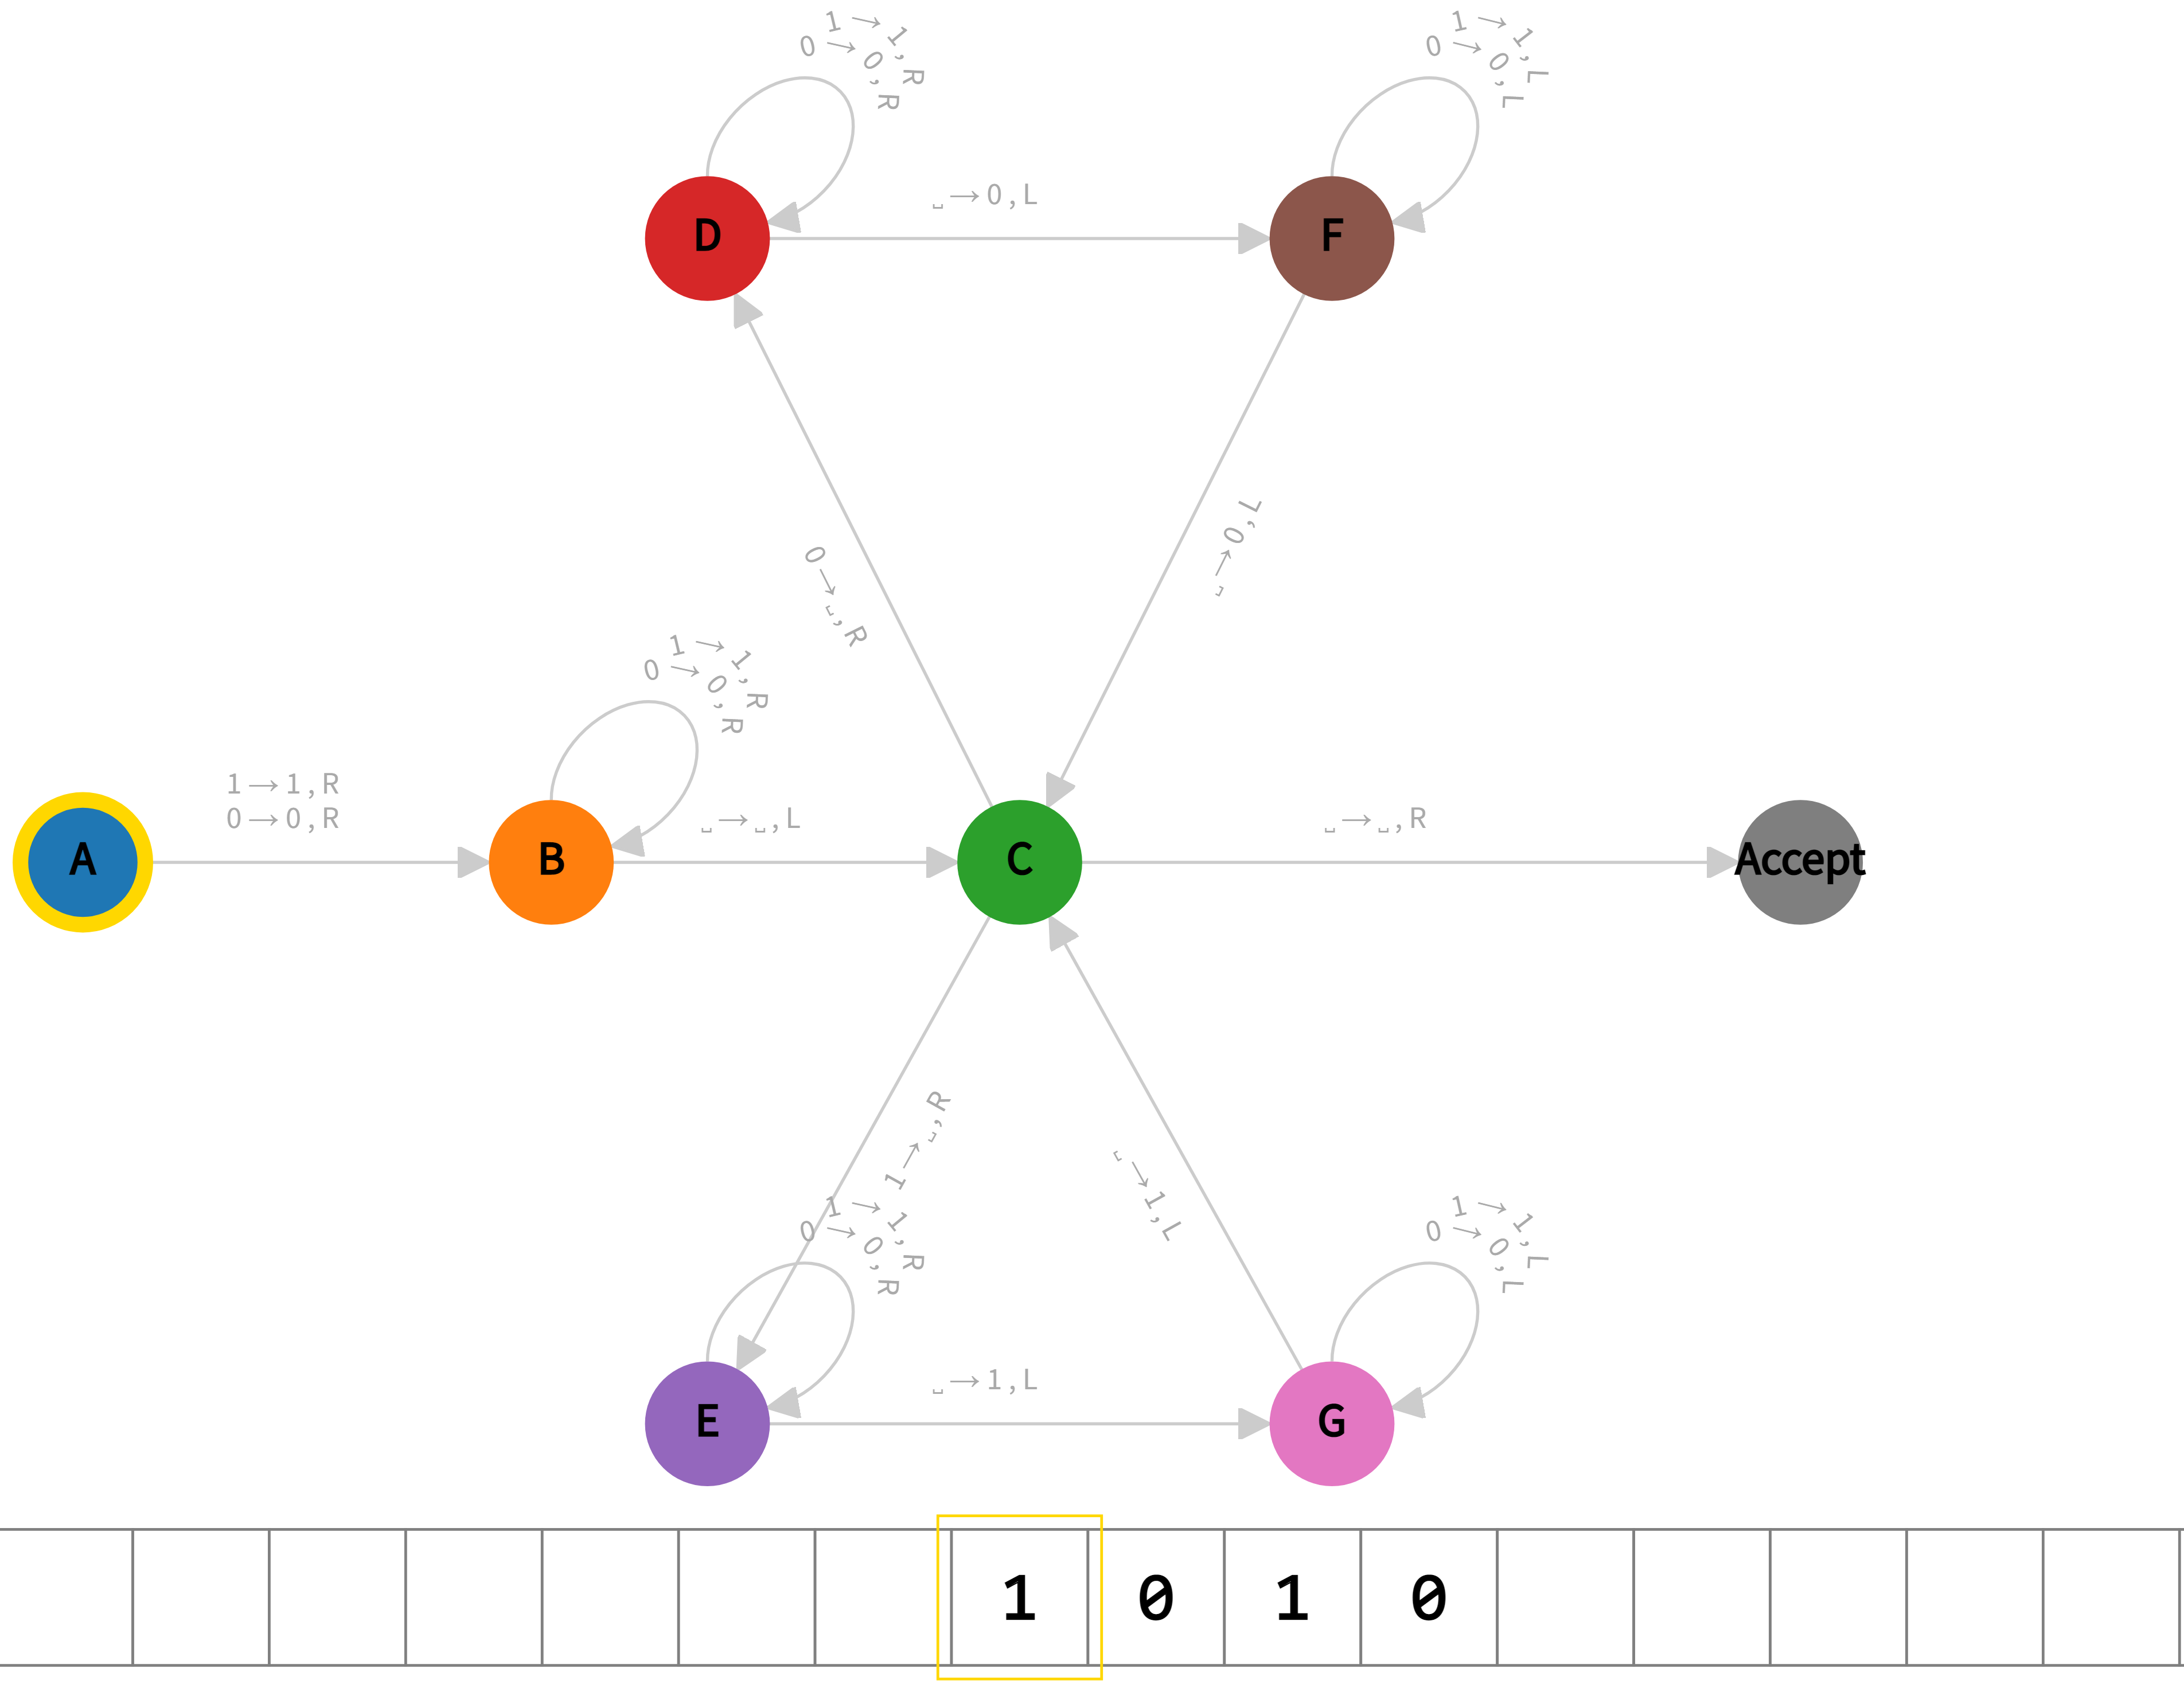
\includegraphics[width=\linewidth]{answers/img/q2-1010-initial.png}
    \caption*{Figure (a): Initial State for $\mathbf{1010}$}
    \label{fig:1010-initial}
  \end{minipage}
  \begin{minipage}{.49\linewidth}
    \centering
    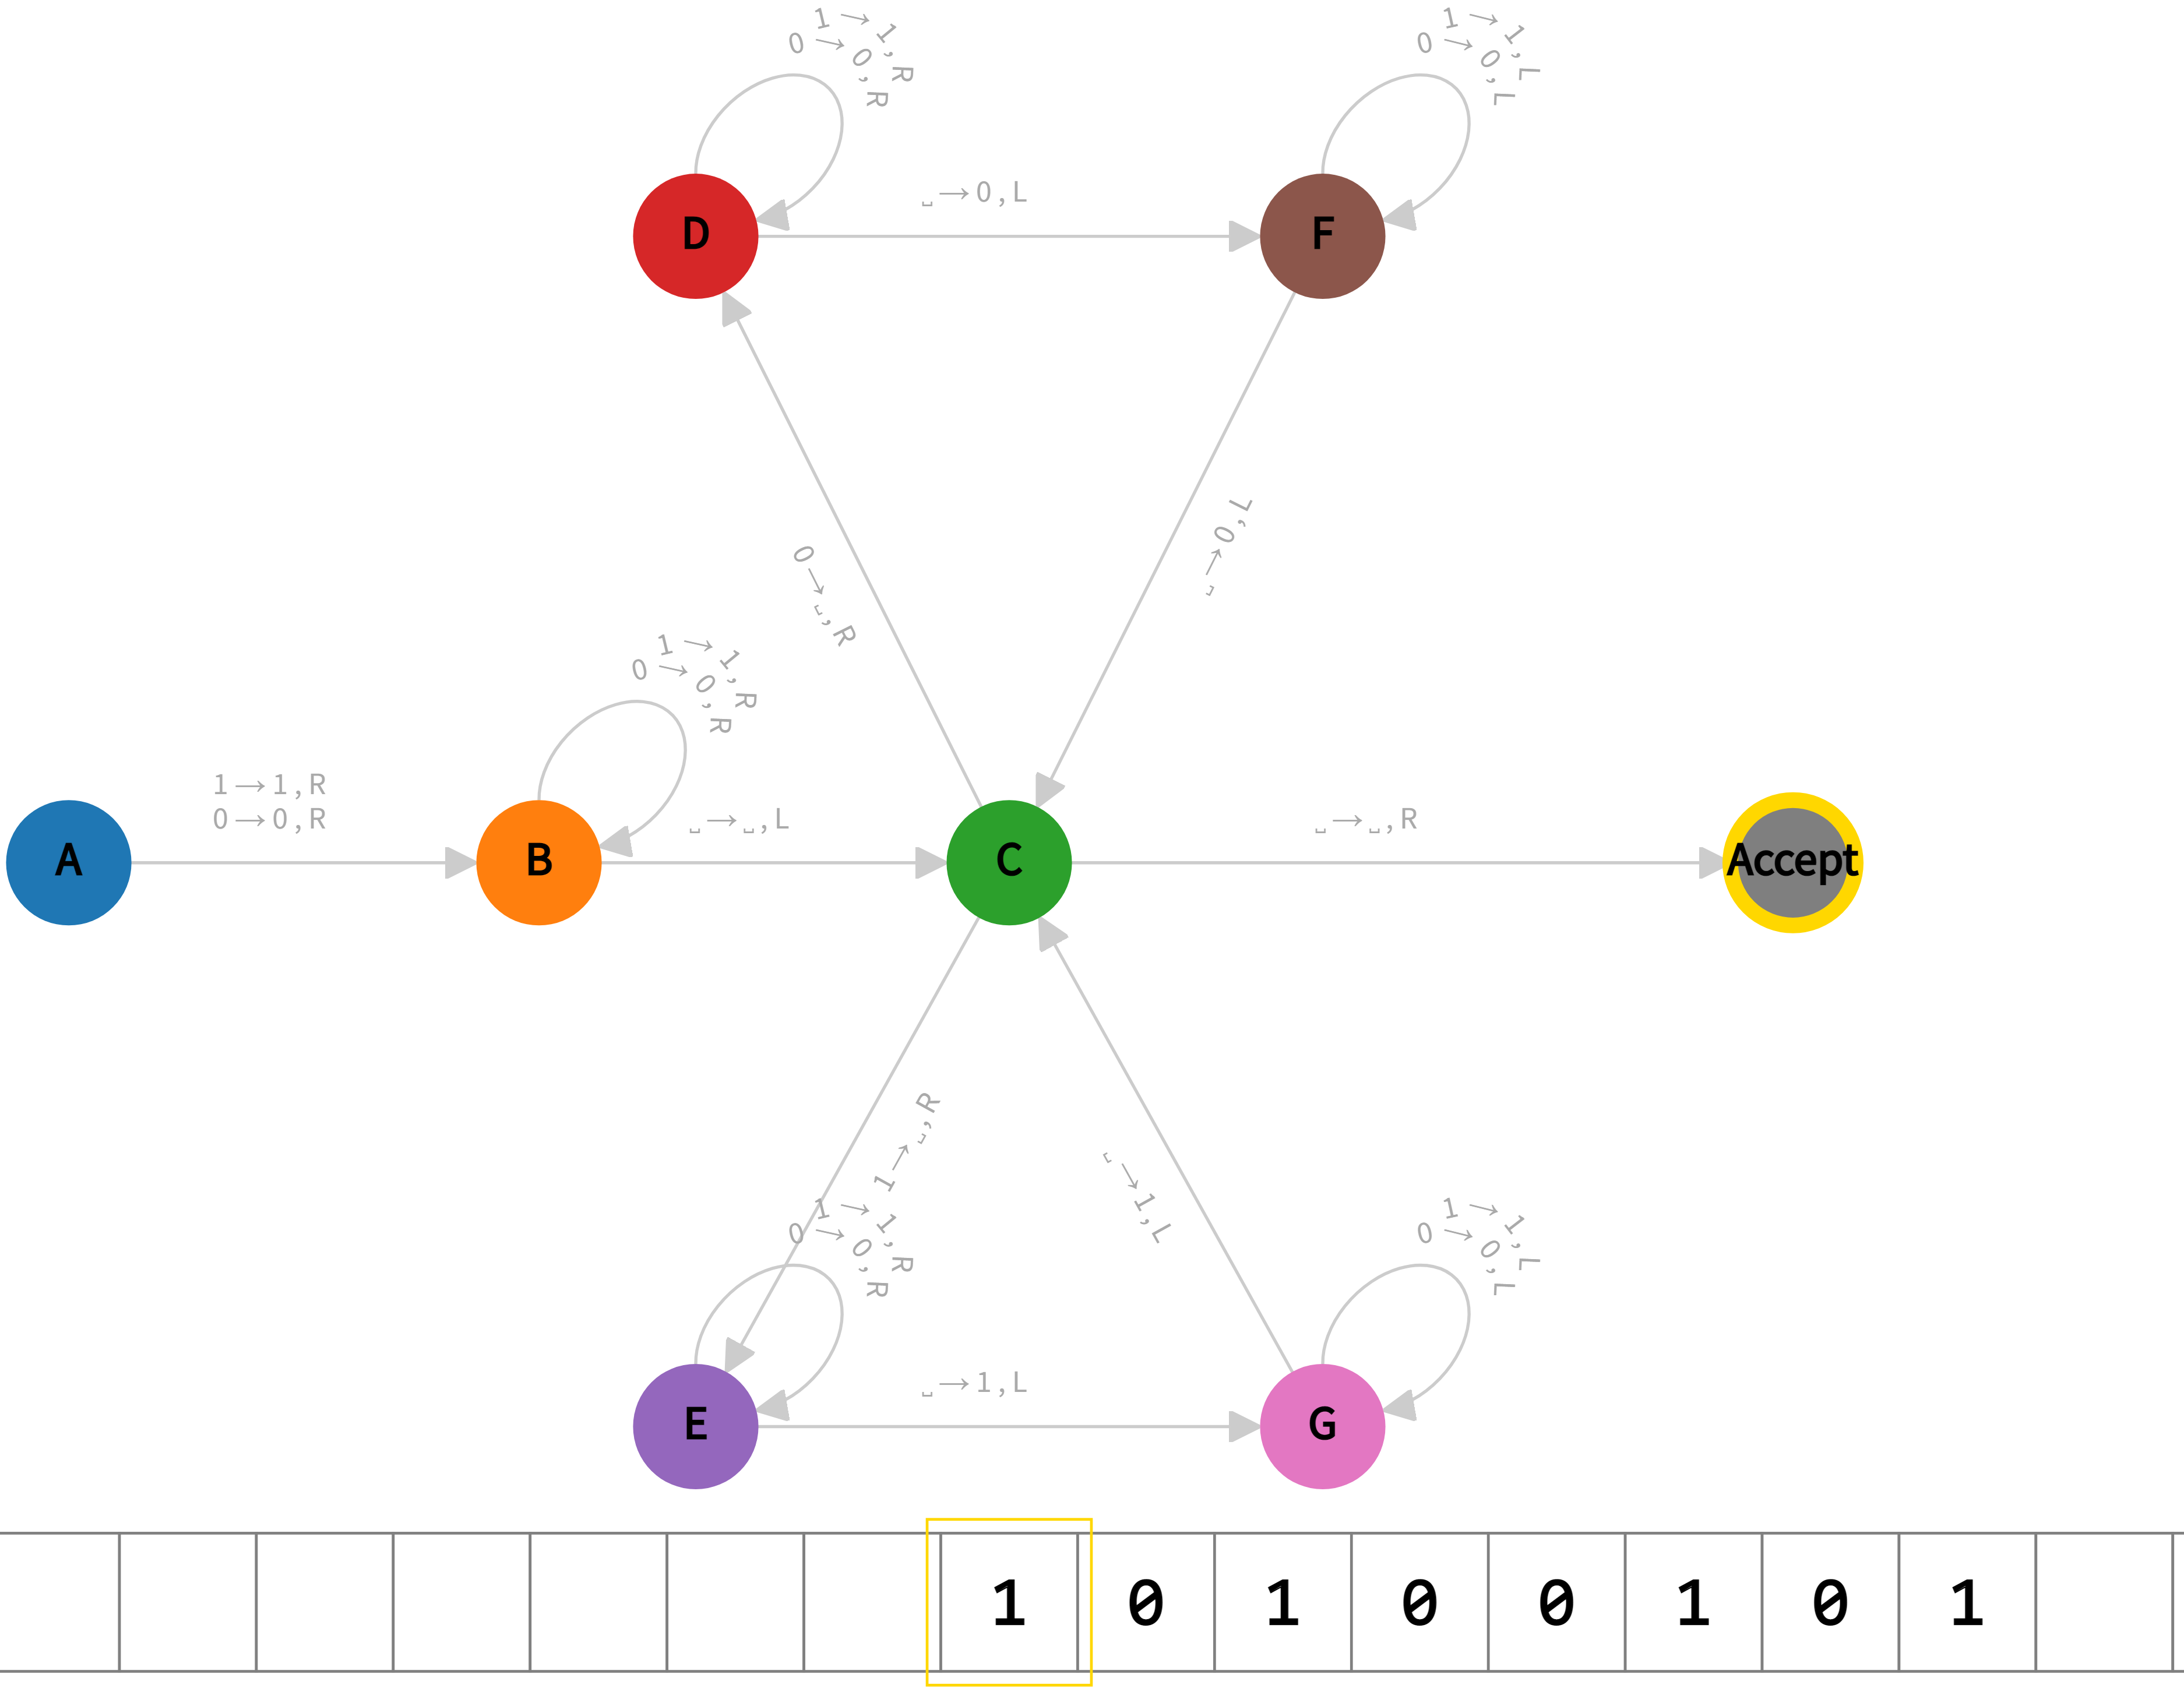
\includegraphics[width=\linewidth]{answers/img/q2-1010-end.png}
    \caption*{Figure (b): End State for $\mathbf{1010}$}
    \label{fig:1010-end}
  \end{minipage}
  \caption{States for $\mathbf{1010}$}
  \label{fig:in-1010}
\end{figure}

\vspace*{\fill}
\newpage
\vspace*{\fill}

\subsection*{Input: 1010001}

\begin{figure}[ht]
  \centering
  \begin{minipage}{.49\linewidth}
    \centering
    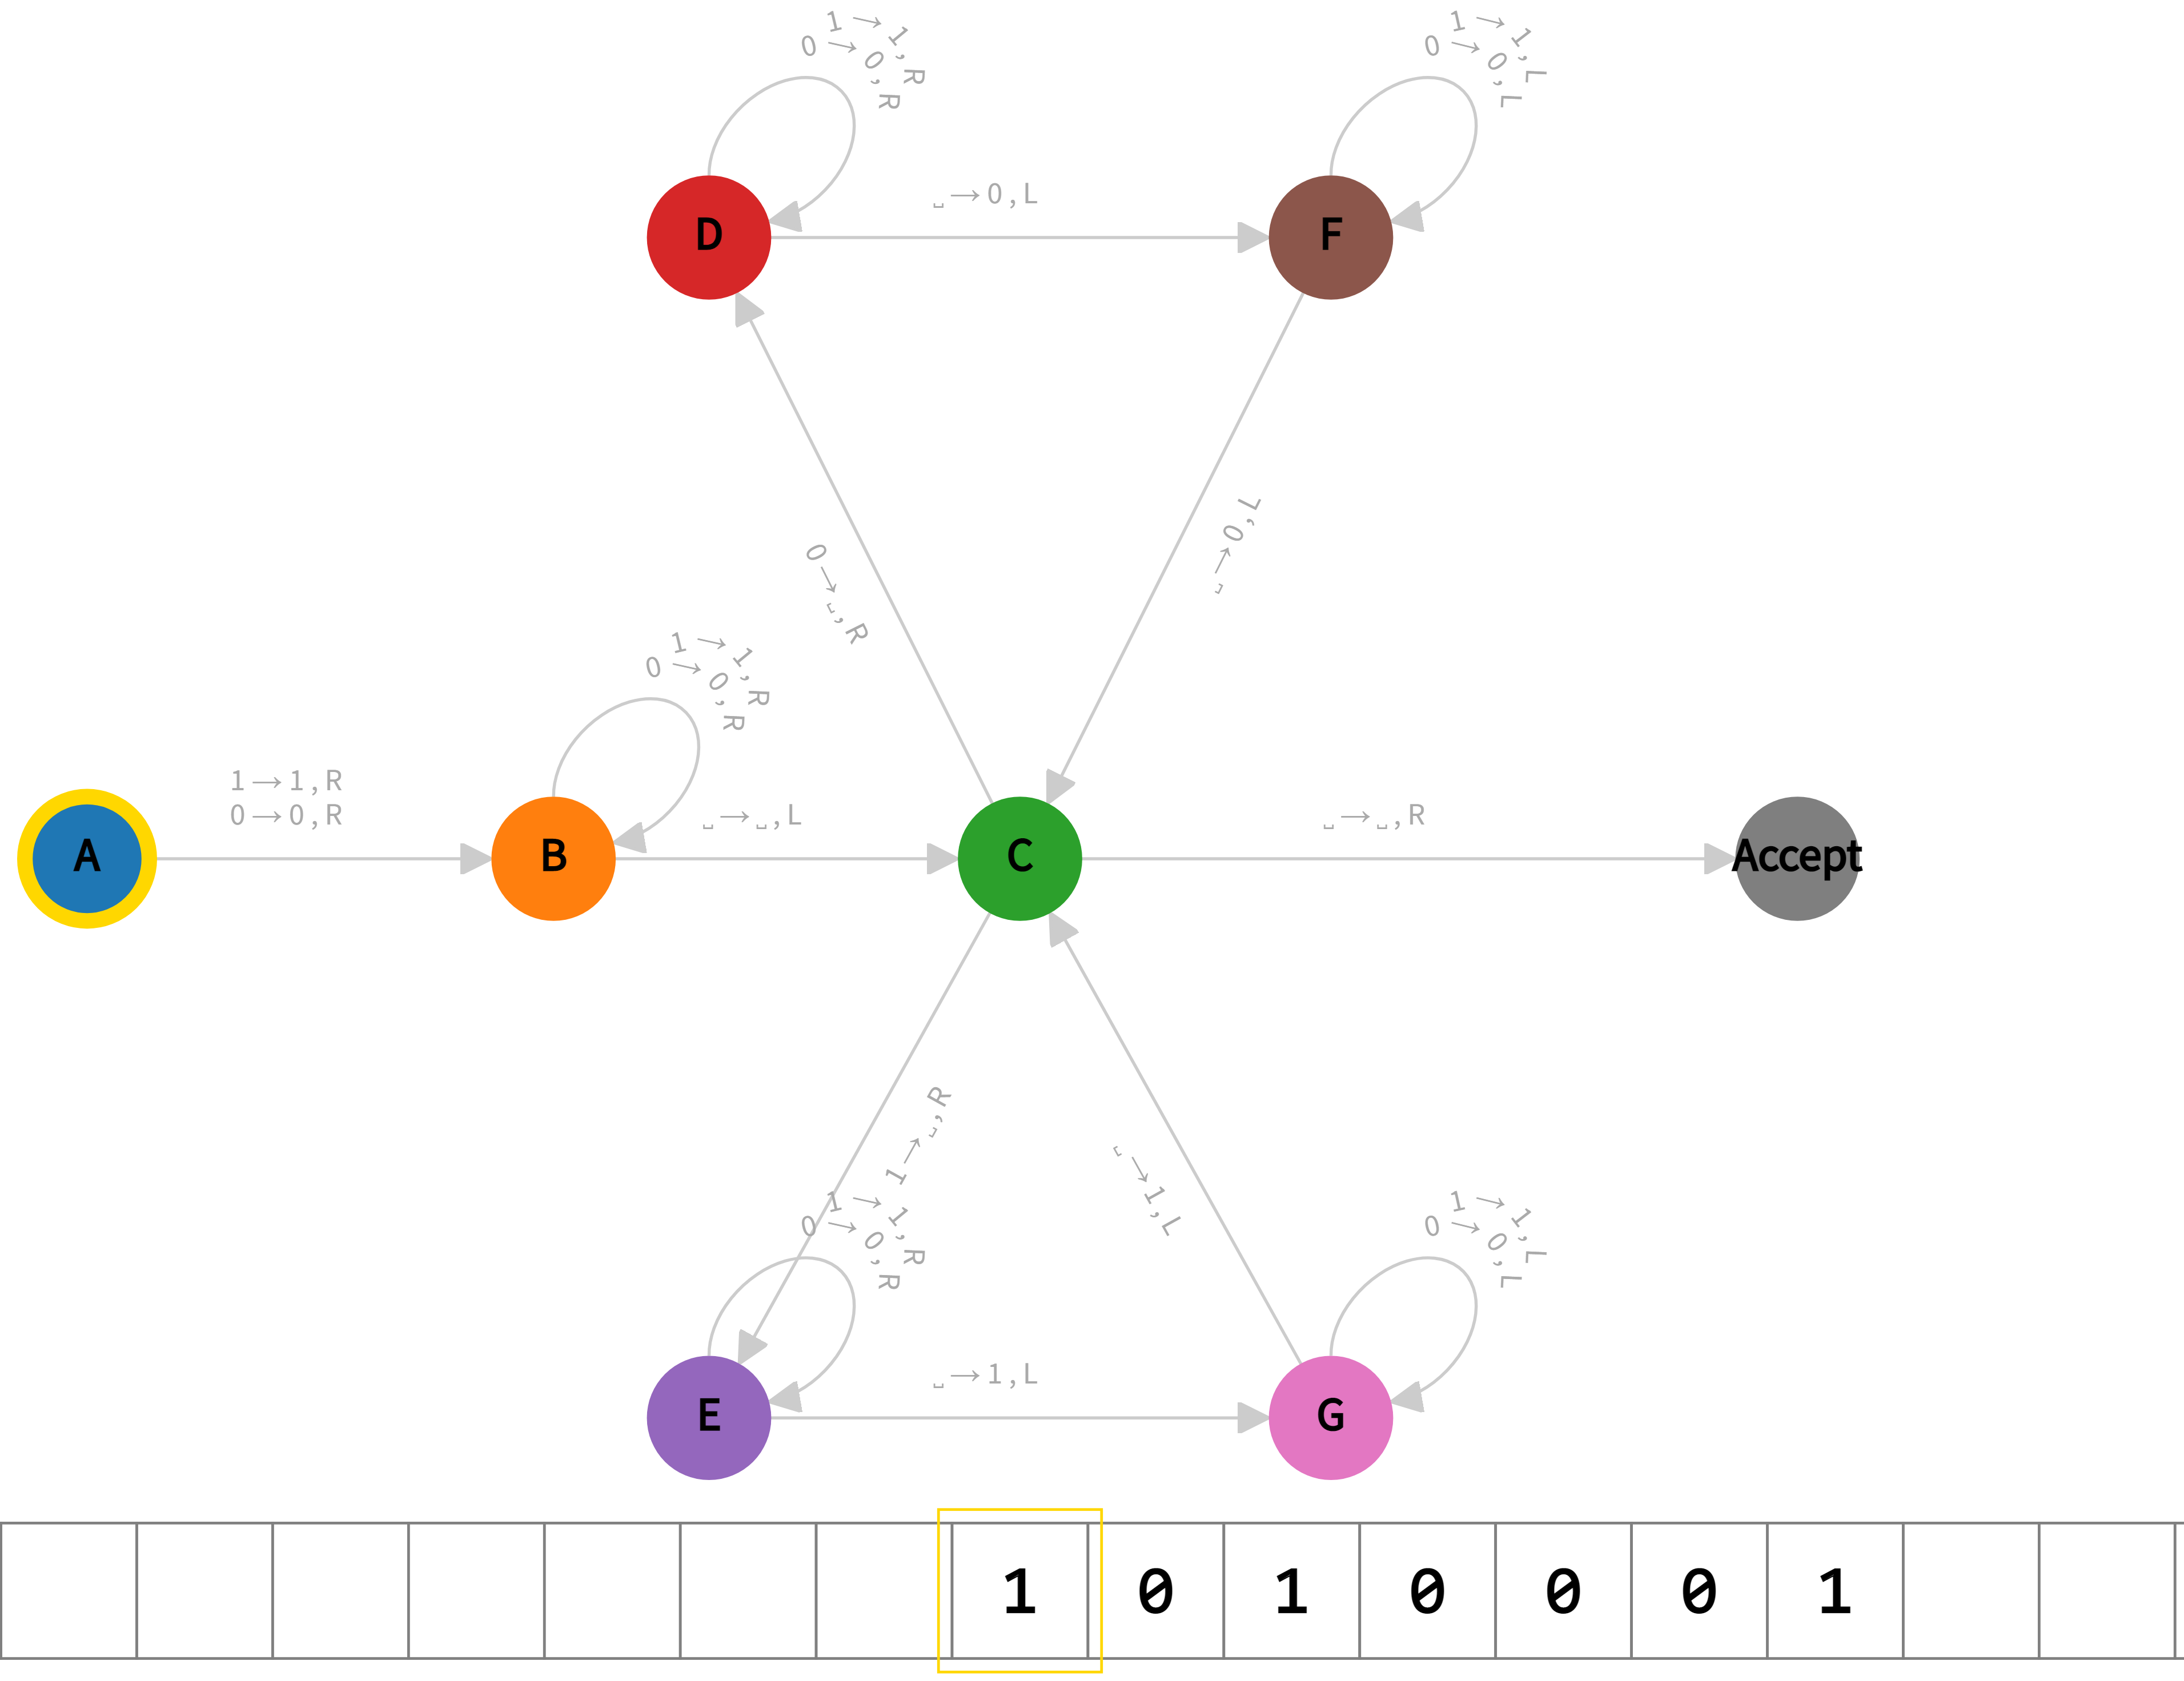
\includegraphics[width=\linewidth]{answers/img/q2-1010001-initial.png}
    \caption*{Figure (a): Initial State for $\mathbf{1010001}$}
    \label{fig:1010001-initial}
  \end{minipage}
  \begin{minipage}{.49\linewidth}
    \centering
    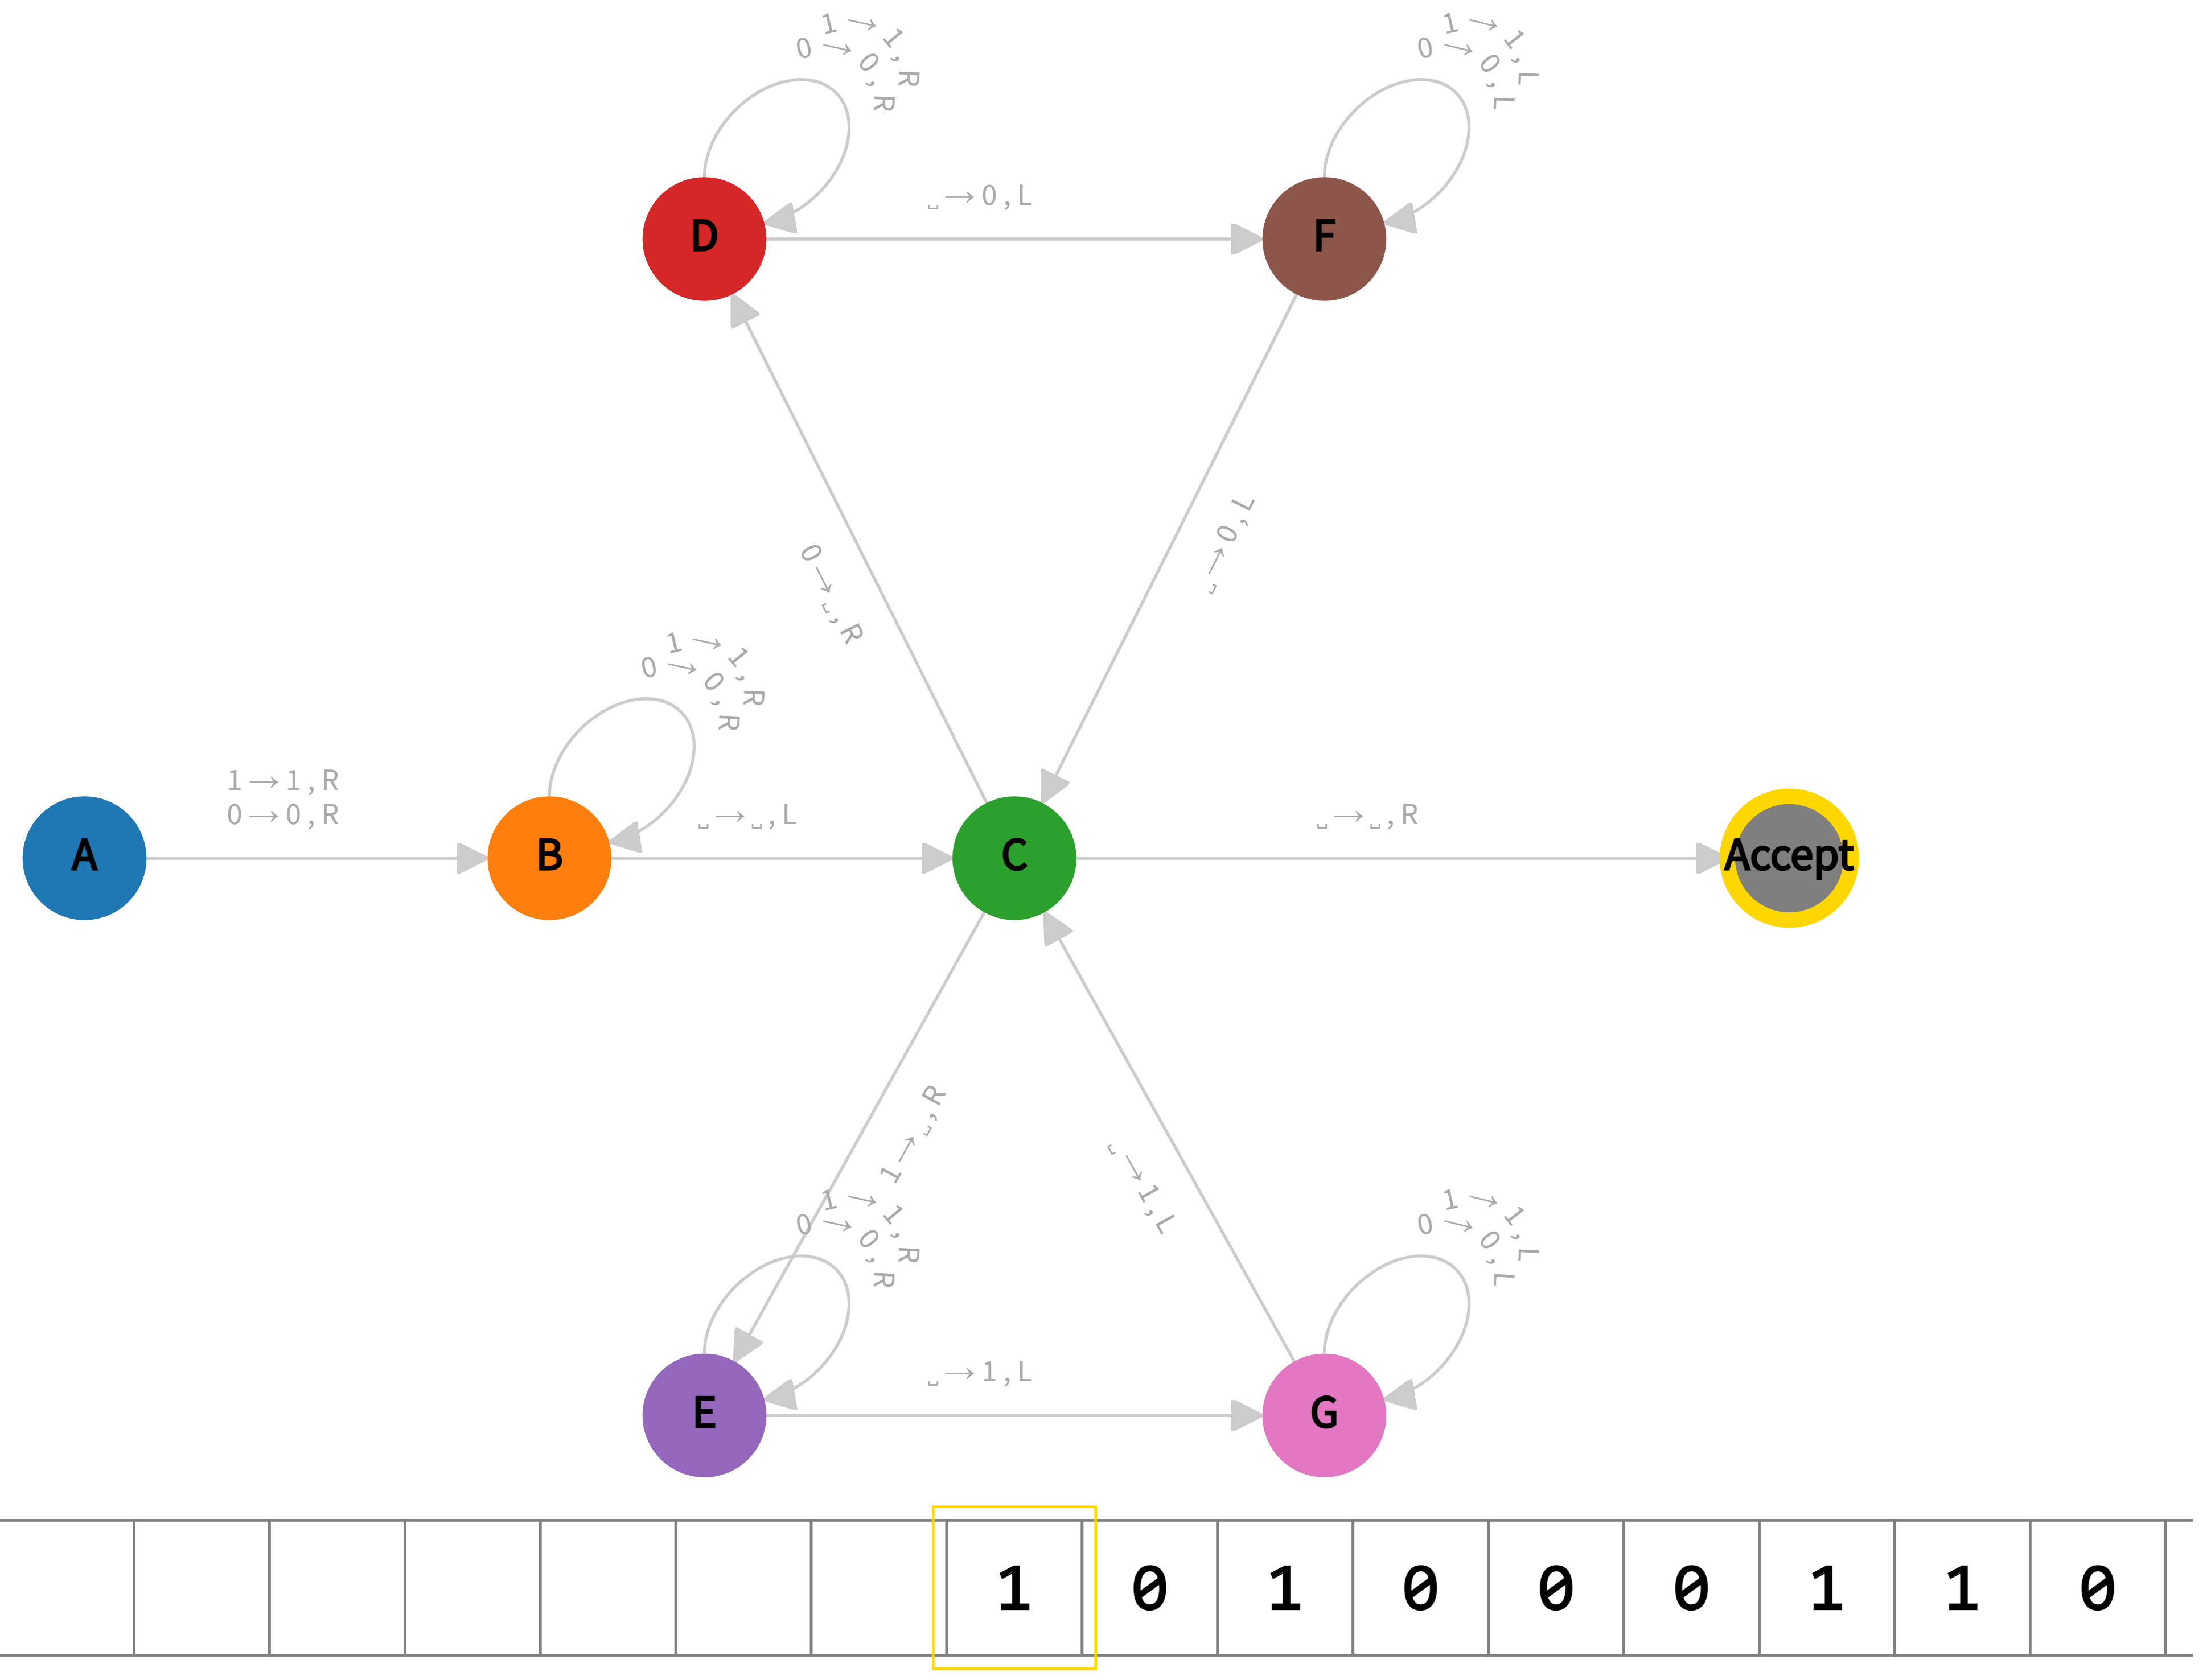
\includegraphics[width=\linewidth]{answers/img/q2-1010001-end.png}
    \caption*{Figure (b): End State for $\mathbf{1010001}$}
    \label{fig:1010001-end}
  \end{minipage}
  \caption{States for $\mathbf{1010001}$}
  \label{fig:in-1010001}
\end{figure}

\begin{center}
\textbf{\textit{Due to the head place, the whole output cannot be seen in \hyperref[fig:1010001-end]{Figure 13.b}.}}
\end{center}

\subsection*{Input: 00111}

\begin{figure}[ht]
  \centering
  \begin{minipage}{.49\linewidth}
    \centering
    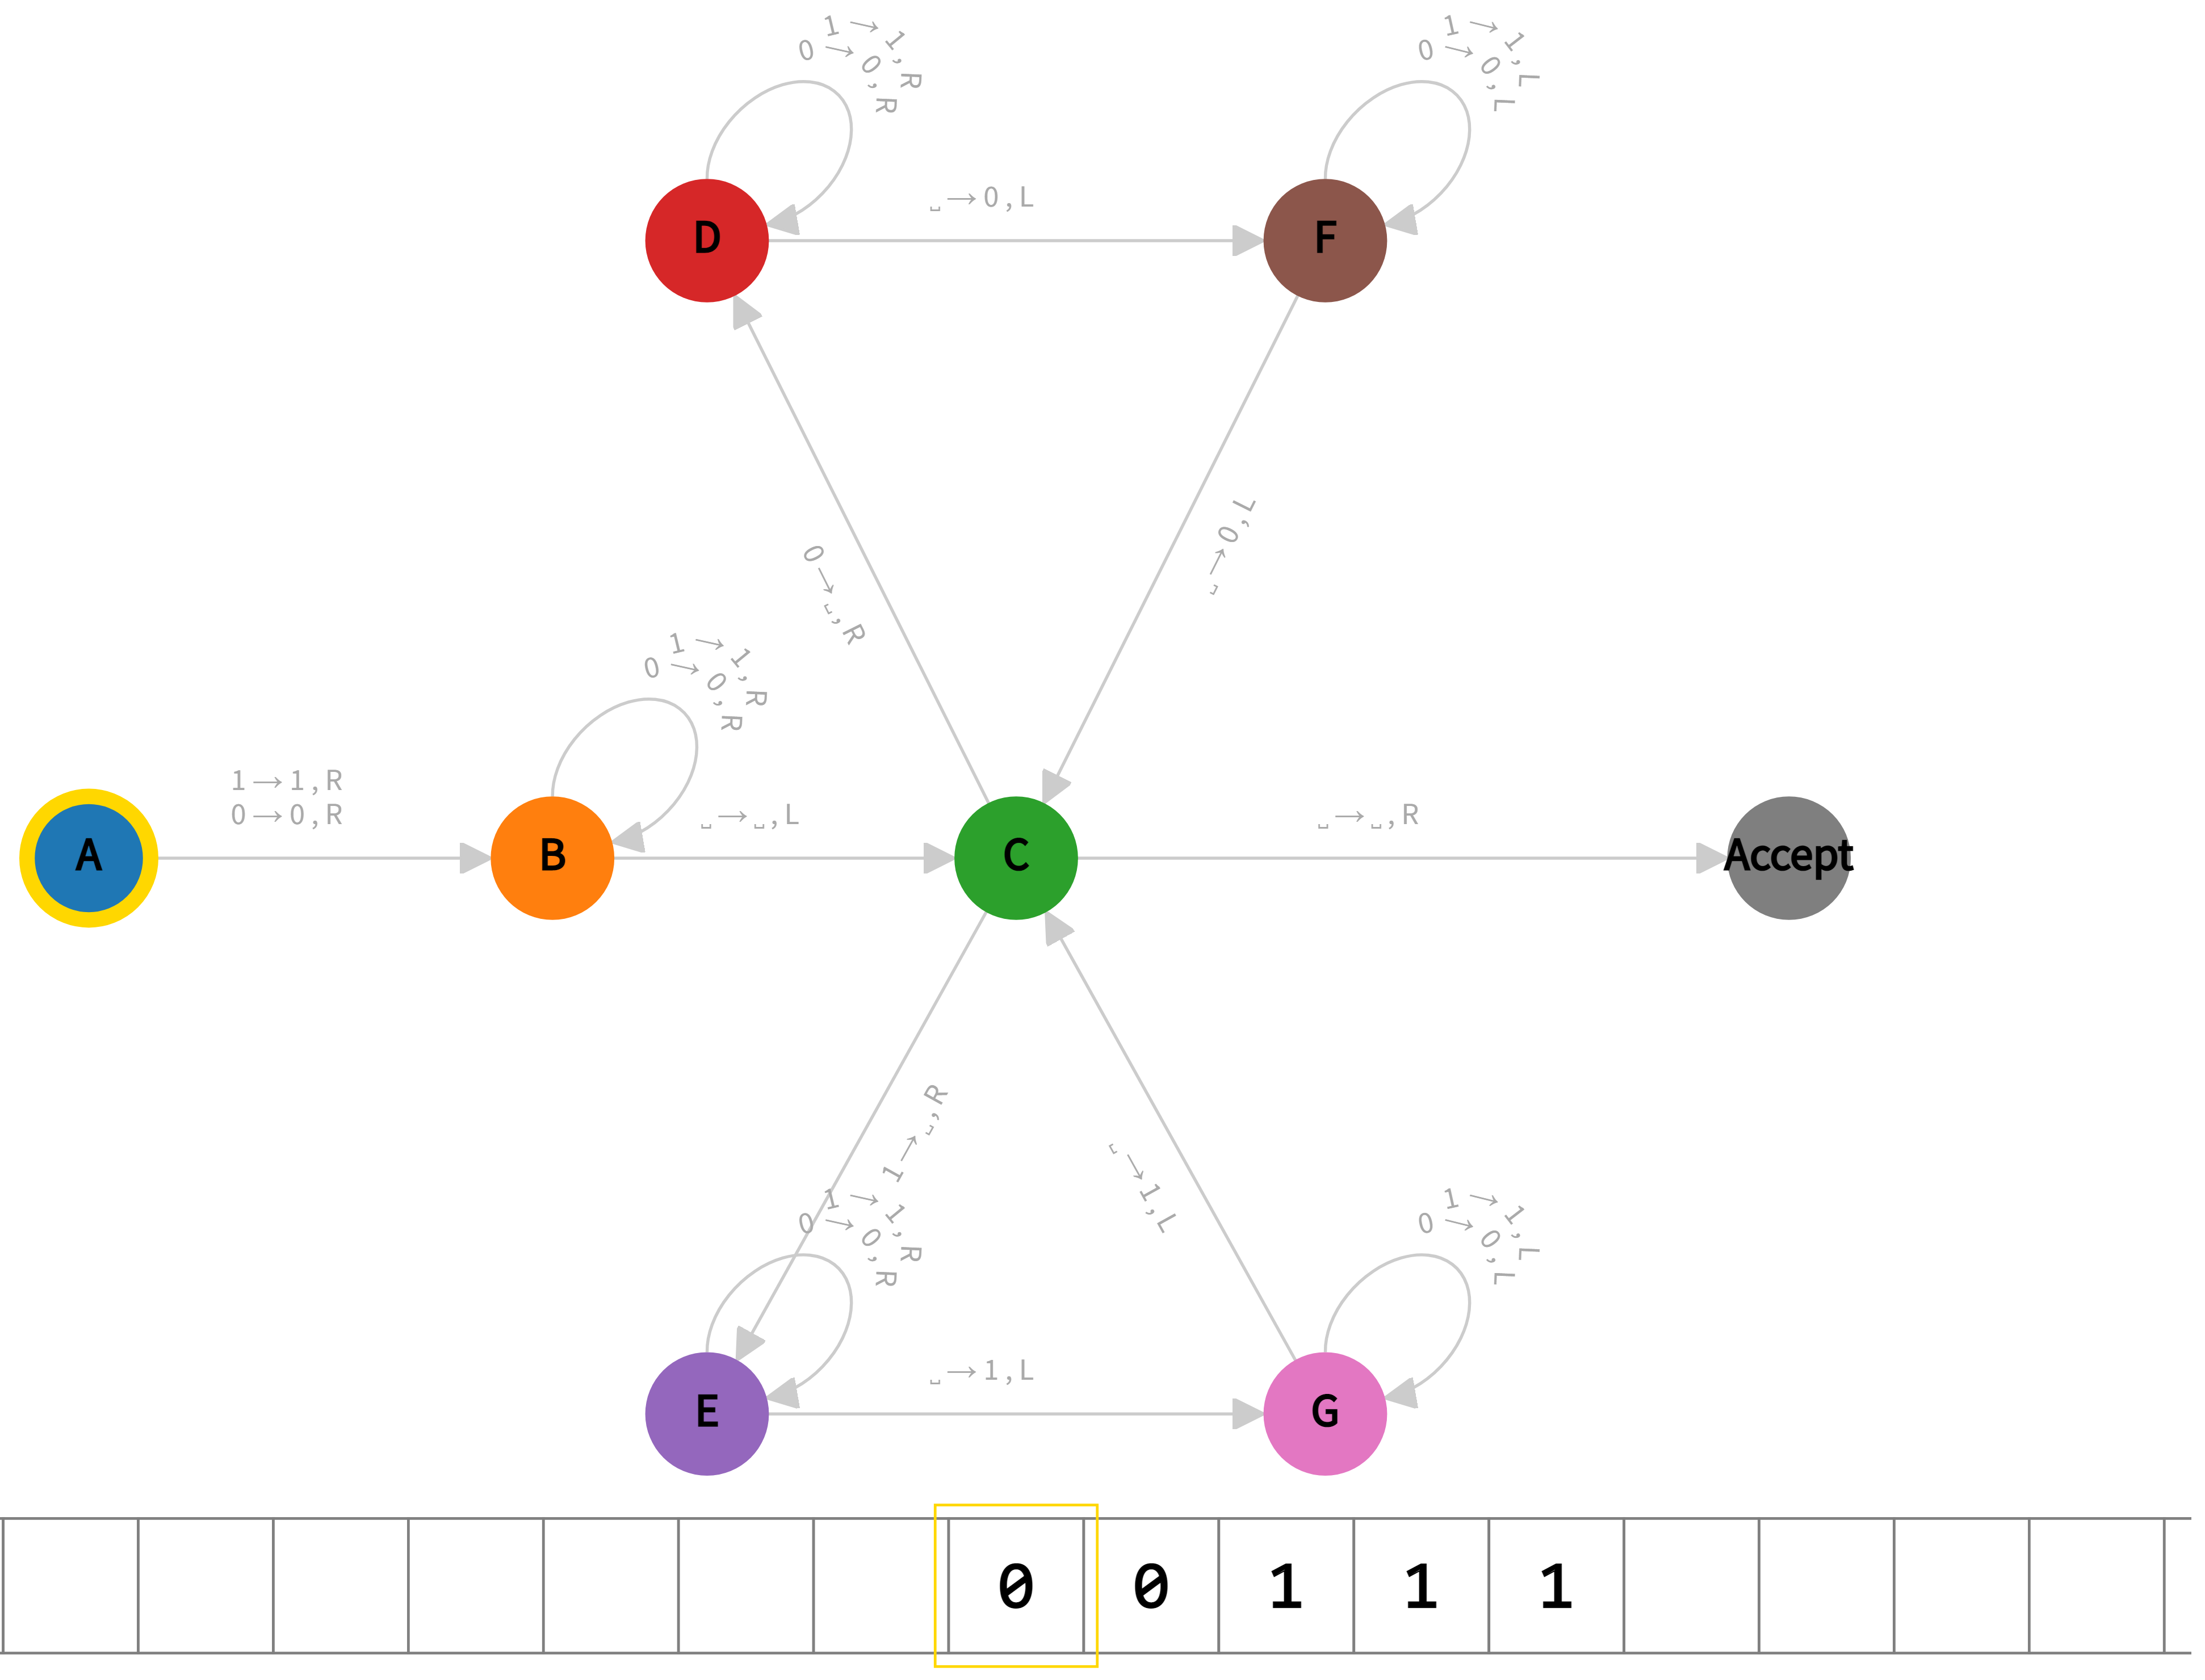
\includegraphics[width=\linewidth]{answers/img/q2-00111-initial.png}
    \caption*{Figure (a): Initial State for $\mathbf{00111}$}
    \label{fig:00111-initial}
  \end{minipage}
  \begin{minipage}{.49\linewidth}
    \centering
    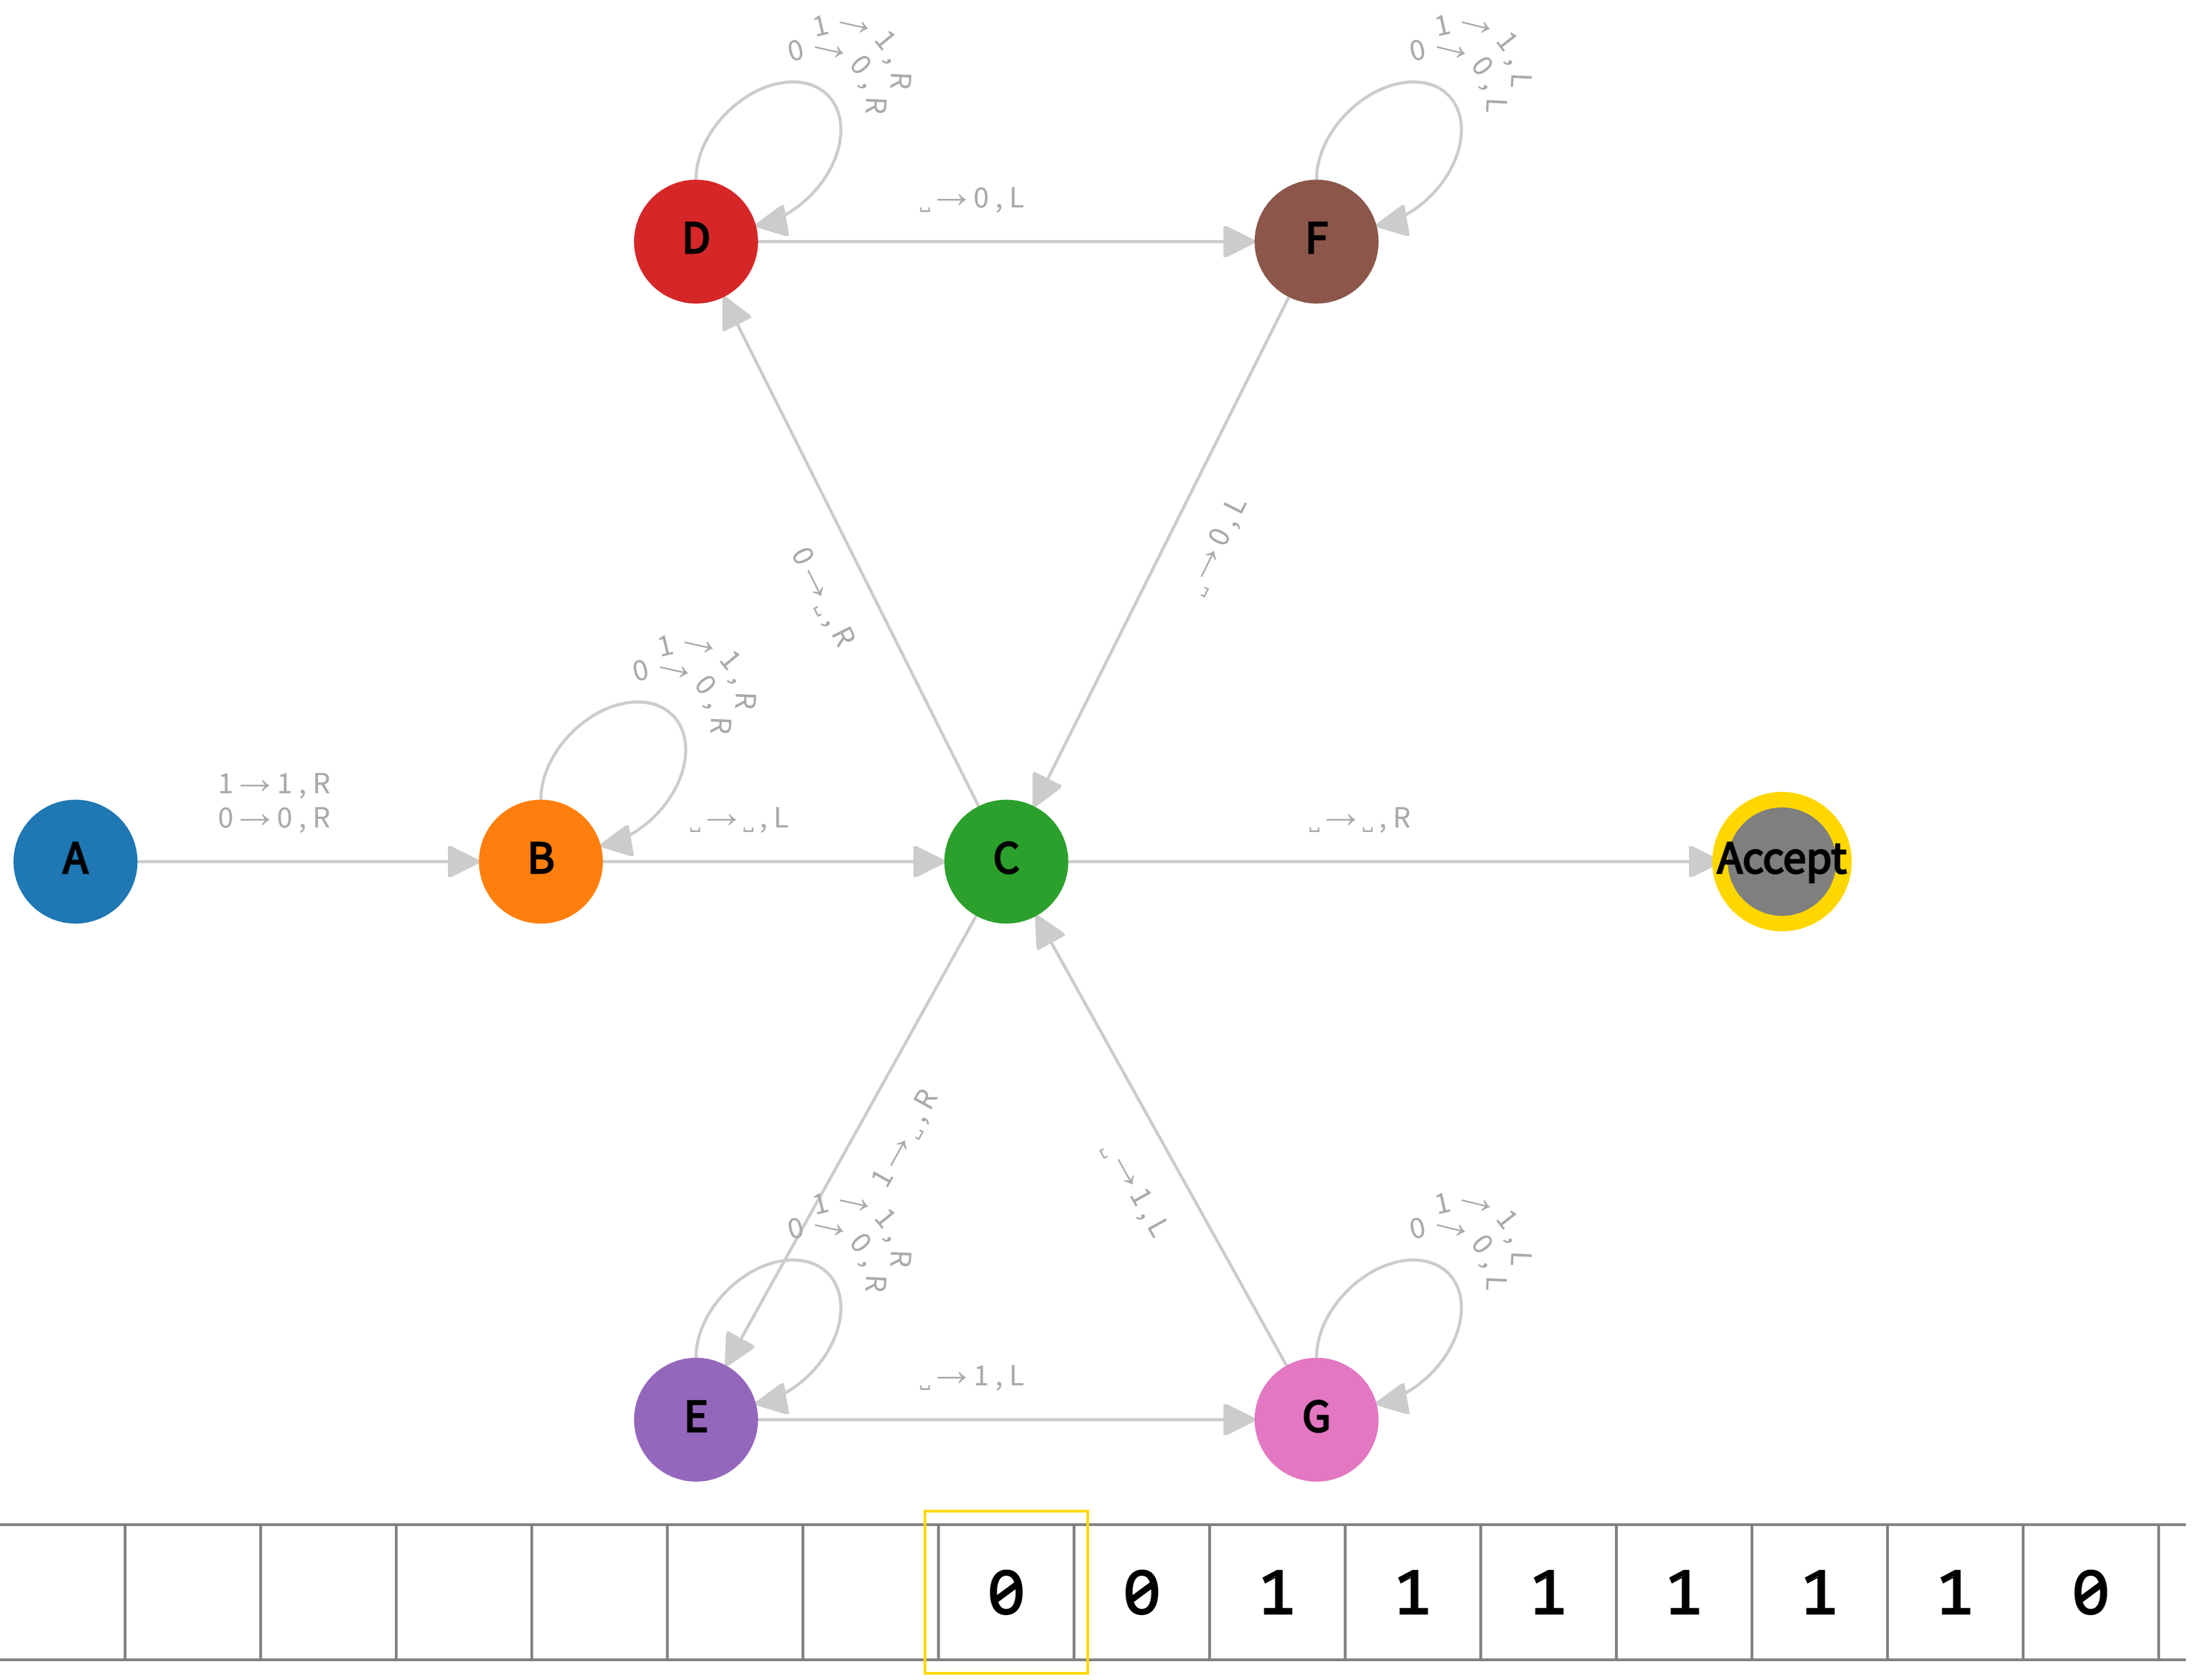
\includegraphics[width=\linewidth]{answers/img/q2-00111-end.png}
    \caption*{Figure (b): End State for $\mathbf{00111}$}
    \label{fig:00111-end}
  \end{minipage}
  \caption{States for $\mathbf{00111}$}
  \label{fig:in-00111}
\end{figure}

\begin{center}
\textbf{\textit{Due to the head place, the whole output cannot be seen in \hyperref[fig:00111-end]{Figure 14.b}.}}
\end{center}

\vspace*{\fill}
\newpage


% General Description

% 1- Scans to the right for first $\blank$. When it is found, move head to left. In other words, find the last symbol in the string.

% 2- Remember the symbol and write $\blank$ and scans to the right for $\blank$. Write symbol to the place instead of $\blank$.

% 3- Scans back to the left for $\blank$ (Lately put). Reinsert the symbol to the place.

% 4- Move head to one left. If it is $\blank$, then stop. If it is a symbol, then repeat 2-4.
